\chapter{RESULTADOS E DISCUSSÃO}

Entender como a contribuição acadêmica influencia na carreira empreendedora dos futuros profissionais das ciências agrárias é de grande interesse para centros acadêmicos, profissionais e educadores. Desta forma, os resultados desta pesquisa encontram-se divididos em seções que atendem aos objetivos propostos no estudo.

Inicialmente são apresentadas descrições que caracterizam os dois perfis estudados (pré-programa e pós-programa Empreenda Agro Sustentável) em relação às variáveis e às comparações entre os grupos. Posteriormente, serão apresentadas as inovações produzidas pelos alunos participantes durante o decorrer do programa.


\section{Alcance da Amostra Experimental do Programa Empreenda Agro Sustentável}

No desenvolvimento do programa foram formadas inicialmente 26 equipes que somaram 118 alunos oriundos dos cursos de graduação do Centro de Ciências Agrárias e Aplicadas da Universidade Federal de Sergipe, além de outros cursos como: artes Visuais, Administração, Design Gráfico, Engenharia Química, Engenharia de Produção, Marketing e Ecologia. Destas 26 equipes inscritas, deram continuidade às propostas durante o programa, 15 equipes. A evasão em projetos educacionais muito antes do início, segundo Ribeiro (2005), pode ser respondida pela falta da cultura de promoção dos modelos educacionais práticos dentro da universidade, assim como projetos que mostrem aos alunos como alavancar seus projetos de vida profissional. Pode contribuir também para a evasão e o interesse dos alunos, a falta de perspectiva de mudança de vida e o distanciamento da cultura empreendedora.
As propostas de negócios se focaram em sua maior quantidade em aplicações mobiles (28,79\%), seguido de negócios para a agricultura sustentável (18,75\%) (Figura \ref{figura_10}). Atualmente muitos aplicativos móveis agrícolas pagos e gratuitos foram desenvolvidos para o meio rural, abrangendo diversas áreas dentro e fora da propriedade rural, trazendo substancialmente contribuição para o desenvolvimento agrícola tanto para grandes propriedades quanto para as menores \cite{silva_caracterizacao_2017}. 
 
\begin{figure}[H]
\caption{\textbf{Número de alunos inscritos e percentual por curso no universo total de participantes do Programa.}}
\centering
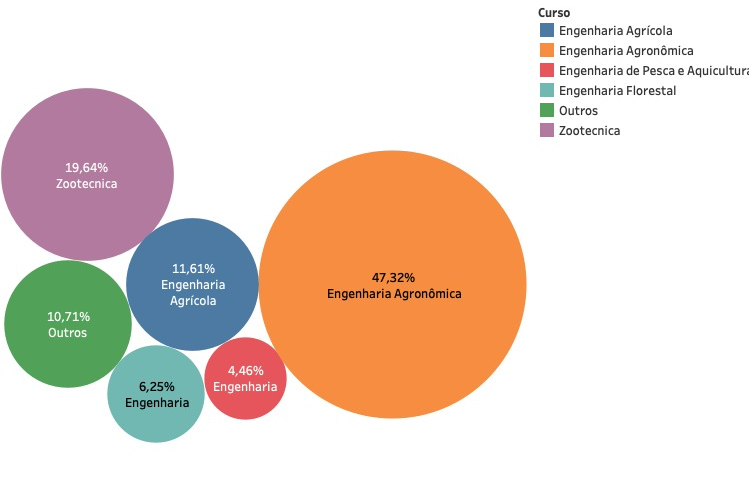
\includegraphics[scale=0.4]{Imagens/inscritos.png}
\fonte{O autor}
\label{figura_10}
\end{figure}

A distribuição da amostra por faixa etária no período de inscrição foi de 75,4\% de estudantes com idade menor que 20 anos, 16,1\% de estudantes com idades no intervalo entre 21 e 25 anos, e 5,9\% tinham idade maior que 25 anos (Tabela \ref{tabela_45}).


\begin{table}[H]
\centering
\caption{\textbf{Faixa etária dos alunos participantes do programa}}
\label{tabela_45}
\begin{tabular}{clcc} 
\hline\hline
 \textbf{Dados}                       & \textbf{Faixa etária}  & \multicolumn{2}{c}{~\textbf{Inscritos} }                                                        \\ 
\hline
\multirow{3}{*}{}                     &                        & \multicolumn{1}{l}{\textbf{Frequência} } & \multicolumn{1}{l}{\textbf{Porcentagem (\%)} }  \\
                                      & \textbf{Menor que 20}  & 89                                            & 75,4                                            \\
                                      & \textbf{De 21 a 25}    & 19                                            & 16,1                                            \\
\multicolumn{1}{l}{\textbf{Válidos} } & \textbf{Maior que 25}  & 7                                             & 5,9                                             \\
\multicolumn{1}{l}{}                  & \textbf{Total}         & 115                                           & 97,5                                            \\ 
\hline
\multicolumn{1}{l}{\textbf{Omissos} } & \textbf{Não informou}  & 3                                             & 2,5                                             \\ 
\hline
\multicolumn{2}{c}{\textbf{TOTAL GERAL} }                      & \multicolumn{1}{l}{118}                       &                                                 \\
\hline\hline
\end{tabular}
\fonte{O autor}
\end{table}


O curso com maior participação numérica foi o de Engenharia Agronômica, representando 47,32\% deste total, enquanto os cursos de Zootecnia, Engenharia Agrícola, Engenharia Florestal e Engenharia Pesca e Aquicultura, participaram em termos percentuais, respectivamente, com 19,64\%, 11,61\%, 6,25\% e 4,46\% do total de estudantes inscritos. O número final de participantes compôs 15 equipes com 3 a 5 estudantes, cada, que transformaram ideias em modelos de negócios, em um processo de capacitação através de metodologias ativas. 

A multidisciplinaridade das equipes contribuiu de forma significativa para o processo criativo, visto que, tal característica é tida como um ponto positivo na elaboração de um modelo de negócio, em que integrantes de diferentes áreas podem conciliar seus conhecimentos e facilitar o processo de criação e desenvolvimento da ideia. Dessa forma, o programa evidenciou a necessidade de propostas que visam explorar esse segmento dentro da universidade, visto que, o empreendedorismo ainda é pouco incentivado no ambiente acadêmico, principalmente dentro das ciências agrárias, a fim de contribuir para a formação de profissionais capacitados para empreender, e com características e conhecimentos que irão destacá-los no mercado de trabalho.

Buscando mitigar estes problemas cada vez mais complexos na produção agrícola, os avanços na agricultura inteligente, métodos de tomada de decisão balizados nas técnicas de informação, agricultura de precisão, e novas tecnologias embarcadas, oferecem ferramentas importantes para enfrentar estes desafios, mantendo a sustentabilidade agrícola. As práticas agrícolas não se concentram apenas no enriquecimento da produtividade agrícola, mas também ajudam a reduzir impactos ambientais prejudiciais de forma sustentável  \cite{adnan_effects_2018,adnan_effects_2018}.

\section{Áreas e Cadeias Produtivas Selecionadas}

A fase de inscrição do programa alcançou 26 propostas de protótipos e/ou negócios na área rural com foco na agricultura sustentável. Na Figura \ref{figura_11} é possível verificar as áreas e cadeias produtivas prioritárias escolhidas. Das quais 15 equipes deram continuidade durante todo o projeto.

As propostas de negócios se focaram em sua maior quantidade em produtos como aplicações móveis (28,79\%), seguido de negócios ligados a agricultura sustentável (18,75\%). Muitos aplicativos móveis agrícolas pagos e gratuitos foram desenvolvidos para o meio rural, abrangendo diversas áreas dentro e fora da propriedade rural. \cite{silva_caracterizacao_2017}. 

\begin{figure}[H]
\centering
\caption{\textbf{Áreas e potenciais propostas de negócios escritos}}
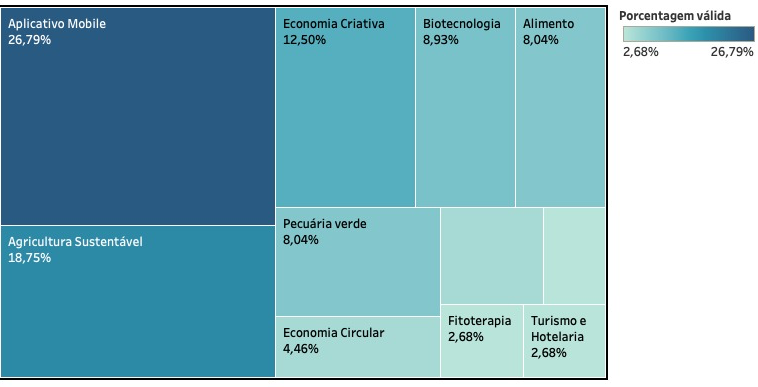
\includegraphics[scale=0.5]{Imagens/propostas_negocios.png}
\fonte{O autor}
\label{figura_11}
\end{figure}

A tecnologia da informação apresenta grandes potencialidades para auxiliar produtores rurais e profissionais da área na tomada de decisões estratégicas, de modo que, o mercado de aplicativos móveis tem tomado força no campo. Todavia, para o profissional das ciências agrárias tomar decisões assertivas, não basta apenas manusear a Tecnologia da Informação aplicada ao agronegócio, é necessário mudar a concepção dos processos a partir de sua informatização \cite{ferraz_tecnologia_2017,sharma_systematic_2020}.

Grandes desafios como a competição de recursos, aumento populacional, competição por terras agricultáveis, representam ameaças à segurança alimentar do planeta, especialmente em países em desenvolvimento e subdesenvolvidos \cite{pardey_bounds_2014}.

Se mostra natural o crescimento do debate sobre a agricultura sustentável, perante as crescentes discussões sobre o paradigma do crescimento da produção de forma sustentável.
\citeonline{rockstrom_sustainable_2017} argumentam que esse paradigma deve ser definido em todas as escalas no contexto atual em que vivemos, de rápidas mudanças ambientais, globais no Antropoceno, ao mesmo tempo que a agricultura  deve se concentrar na erradicação da pobreza e da fome e contribuir para o bem-estar humano.

Buscando mitigar estes problemas cada vez mais complexos na produção agrícola, os avanços na agricultura inteligente, métodos de tomada de decisão balizados nas técnicas de informação, agricultura de precisão, e novas tecnologias embarcadas, oferecem ferramentas importantes para enfrentar estes desafios, mantendo a sustentabilidade agrícola. As práticas agrícolas não se concentram apenas no enriquecimento da produtividade agrícola, mas também ajudam a reduzir impactos ambientais prejudiciais de forma sustentável \cite{adnan_effects_2018,rockstrom_sustainable_2017,ye_bio-organic_2020}.

\section{Avaliação do Questionário Aplicado}

Para a análise do questionário aplicado neste survey, foi utilizado o teste de confiabilidade e agrupamento dos dados amostrais por rotação Varimax, tendo como dados de normalização o Kaiser\footnotemark[1]. Após análise estatística, emergiram 3 componentes principais esperados para esta pesquisa, aglutinando as questões na ordem apresentada no apêndice \ref{chap:tabela_2}.


As questões \textbf{“Para mim sem empresa não é autônomo”} e \textbf{“Pensando em todos os possíveis recursos que minha família me fornece, eu sou completamente dependente dela para decidir como alocá-los e usá-los”}, foram eliminadas da pesquisa, os argumentos acadêmicos defendem que a mesma variável não pode contribuir para a construção de fatores distintos. Desta forma, nesta pesquisa foi adotado o valor 0,40 como limite aceitável da contribuição da variável na criação do fator, com o objetivo de evitar o problema da indeterminação da relação entre variáveis e fatores \cite{figueiredo_filho_visao_2010}. Valores de demais questões podem ser observados no  Apêndice \ref{chap:tabela_2}. 



%A tabela \ref{tab:tabela_4} apresenta a variância total explicada para as dimensões tratadas na pesquisa.
%\begin{table}[H]
% \centering
%\caption{\textbf{Variância total explicada}}
%\label{tab:tabela_4}
%\hline\hline
%\begin{tabular}{c c c c }
%multicolumn{1}{p{6cm}}{} & \multicolumn{3}{c}{\textbf{Fatores}}\\ 
%\multicolumn{1}{c}{\textbf{Itens}} & \multicolumn{3}{c}{\hrulefill}\\ 

%\multicolumn{1}{c}{} 
%&\multicolumn{1}{c}{\textbf{Autoeficácia}} & %\ulticolumn{1}{c}{\textbf{Intenção}} &\multicolumn{1}{c}{\textbf{Família}}  
%\\\\ \hline 

% Somas de rotação de carregamentos ao quadrado (n)
% & 6,602 & 4,090 & 2,802 \\\\
% Variância explicada (\%)
% & 22,766 & 14,102 & 9,662\\\\
% Variância cumulativa (\%)
% & 22,766\% & 36,868\% & 46,530\% \\\hline \hline 
%\end{tabular}
%\fonte{O autor}.
%\end{table}


O questionário resultante da rotação Varimax, o teste de esfericidade de \textit{Bartlett} demonstrou haver significância e validade dos resultados já que a significância dos dados obtidos foram menores que 0,05\%, demonstrando haver ajuste dos dados à Análise Fatorial Exploratória (AFE), desta forma, os dados satisfazem o objetivo proposto na pesquisa, desde que para as análises posteriores sejam utilizados testes não paramétricos, para isto foram utilizados na análise de distribuição o método \textit{Kolmogorov-Smirnov}, da mesma forma para os testes post-hoc foi utilizado o teste U de \textit{Mann-Whitney} Tabela \ref{tabela_8}.

Resultados abaixo de 0,5 indicam que a análise fatorial é insatisfatória em decorrência da baixa correlação entre as variáveis. Valores da estatística KMO acima de 0,6 confirmam a validade dos dados coletados. Na realização do teste KMO dos dados levantados, foram obtidos os resultados que seguem para os momentos do experimento na Tabela \ref{tabela_8}.

\begin{table}[H]
\FloatBarrier
\centering
\caption{\textbf{Estatística KMO e Bartlett para o questionário}}
\label{tabela_8}
\begin{tabular}{ll|l}
\hline\hline
\multicolumn{2}{l|}{\multirow{2}{*}{Medida KMO de adequação da amostragem.}} &  \\
\multicolumn{2}{l|}{} & ,604 \\ \hline
\multirow{3}{*}{Teste de esfericidade} & Aprox. Qui-quadrado & 1041 \\
 & \\
 & \textit{P-valor}. & ,000 \\ \hline
\end{tabular}
\fonte{O autor}
\end{table}

\section{Resultado da Análise do Survey Aplicado}

Este trabalho considerou quatro possíveis conjuntos de variáveis que influenciam na resposta da educação em empreendedorismo. Diversos autores abordam diferentes pontos sobre esta temática, visto que este programa se comporta como uma fase de pré-aceleração, foram estudadas as seguintes dimensões: a dimensão da autoeficácia dos estudantes,  a dimensão familiar e influência de terceiros no desenvolvimento empreendedorismo e dimensão da intenção  ao empreendedorismo dos estudantes.


%\subsection{Interesse em conteúdos relacionados a educação em empreendedorismo}


%Como mostra a Tabela 1, os estudantes participantes do programa se caracterizam por uma maior diferença entre
%gostaria de fazer e não tenho interesse em fazer do que os pesquisados por  \cite{lima_ser_2015} no Brasil. A única exceção ocorre para com empreendedores experientes. Quanto à disciplina de empresas familiares, no contexto da educação em empreendedorismo, ela parece reforçar a sinalização já feita pelos estudos do CFA (Andrade et al., 2006; Mello et al., 2011) da necessidade de conteúdo de formação em administração de micro e pequenas empresas.


\subsection{Dimensão Autoeficácia Empreendedora}

Considerando que os escores das perguntas relacionadas à dimensão empreendedora varia de 1, menor número, a 7, maior número na escala, foi avaliada a média de cada variável (questão). O histograma (Figura \ref{figura_autoeficacia}) foi extraído partindo da mediana de cada respostas aglutinadas em fatores, em que quanto mais próximo de 7, melhor a perspectiva de mudança positiva para a amostra pesquisada. Foi observado, utilizando o Wilcoxon Signed pareado com o intervalo de confiança em 95\%, que a autoeficácia para os participantes, sem considerar as diferenças dos cursos, não variou significativamente (p-valor 0,118), porém, observando as médias nos histogramas das respostas antes e após a participação do programa passou de 5,31 para 5,65 (Figura \ref{figura_autoeficacia}) e que as respostas aumentaram a frequência para os quesitos 6 \textit{"Seguro"} e 7 \textit{"Completamente seguro"}.

A autoeficácia empreendedora é uma importante dimensão para a geração de inovação e criatividade para novos negócios e produtos escaláveis. \citeonline{gubik_student_2016} afirmam que a autoeficácia relacionada ao empreendedorismo e ao conhecimento de processos empresariais também afetam significativamente as intenções empresariais, e que, alunos mais autoconfiantes (maior lócus de controle) têm maior autoeficácia e em consequência melhor desempenho nos negócios.

Neste sentido, as instituições de ensino superior, independente da ciência de estudo, devem ser capazes de proporcionarem atividades didáticas que tenham como propósito a melhoria do nível da autoeficácia dos alunos resultando numa melhora das competências empreendedoras após a formação deles \cite{ribeiro_autoeficacia_2019}. A busca pela melhoria da dimensão da autoeficácia empreendedora ajudará a moldar o futuro dos alunos no mercado de trabalho e motivará a ter sucesso em seus futuros negócios, permitindo assim aos alunos definirem e seguirem seus próprios percursos profissionais com sucesso \cite{das_examining_2018}.

\begin{figure}[H]
\centering
\caption{\textbf{
Contagem dimensão da autoeficácia empreendedora  por momento da pesquisa}}
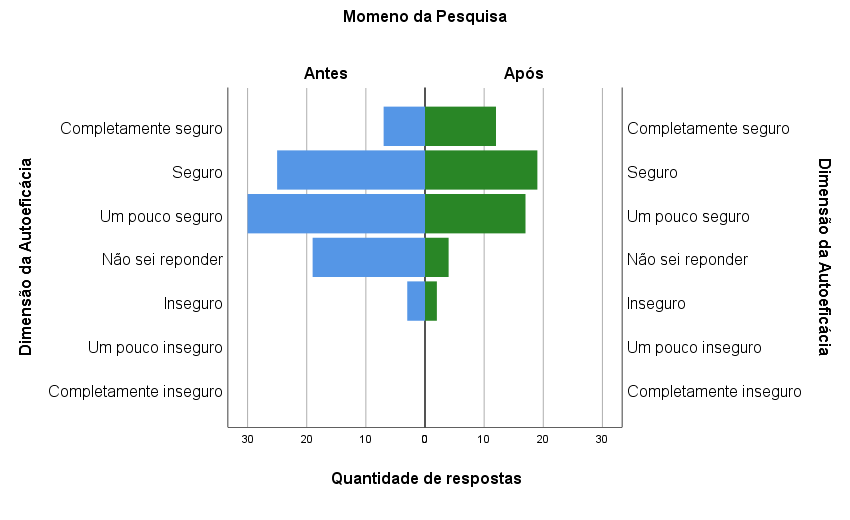
\includegraphics[scale=0.5]{Imagens/dimensao_autoeficacia.png}
\fonte{O autor}
\label{figura_autoeficacia}
\end{figure}


Por meio da análise do gráfico Box Plot (Figura \ref{figura_34}) é possível observar que os cursos de Engenharia Agrícola, Engenharia Agronômica, Engenharia Florestal e Zootecnia possuem acadêmicos mais seguros após a participação no programa.

Para os alunos vinculados ao curso de Engenharia Agrícola é possível observar uma significativa mobilidade positiva no 2º e 3º quartis, em que as afirmações “Um pouco seguro” (5,00) e “Seguro” (6,00), passaram para “Seguro” (6,00) e “Completamente seguro” (7,00), demostrando que o programa influenciou positivamente os alunos deste curso.  

O curso de engenharia Agronômica também apresentou mudança positiva observada no 2º quartil em que a afirmação “Um pouco seguro” (5,00) passou para “Seguro” (6,00). No entanto, não houve mudança para o 3º quartil localizado entre as afirmações “Um pouco seguro” (5,00) e “Seguro” (6,00). Além disso, foi observada uma redução dos resultados abaixo da afirmação “Um pouco seguro” (5,00). Outro fator observado foi a significativa diminuição de respostas na afirmação “Inseguro” (3,00). Estes dados demonstram que os alunos deste curso se sentiram menos inseguros após a participação no programa.
Por ser um curso com poucos participantes, o curso de Engenharia de pesca apresentou uma mudança positiva dos resultados, porém sem variação entre os quartis observados.

O curso de Zootecnia apresentou uma alta dispersão nos resultados pós-programa, porém quando observado o 2º quartil localizado entre as afirmações “Não sei responder” (4,00) e “Um pouco seguro” (5,00), a frequência na afirmação “Não sei responder” se anulou, ficando os dados concentrados na afirmação “Um pouco seguro” (500).


Para os demais cursos que participaram da pesquisa, foi observada uma mobilidade positiva do 2º quartil que estava localizado entre a afirmação “Um pouco seguro” (5,00) e “Seguro” (6,00), para a afirmação “Seguro” (5,00).


\begin{figure}[H]
\centering
\caption{\textbf{Mobilidade da autoeficácia antes e após o programa por curso}}
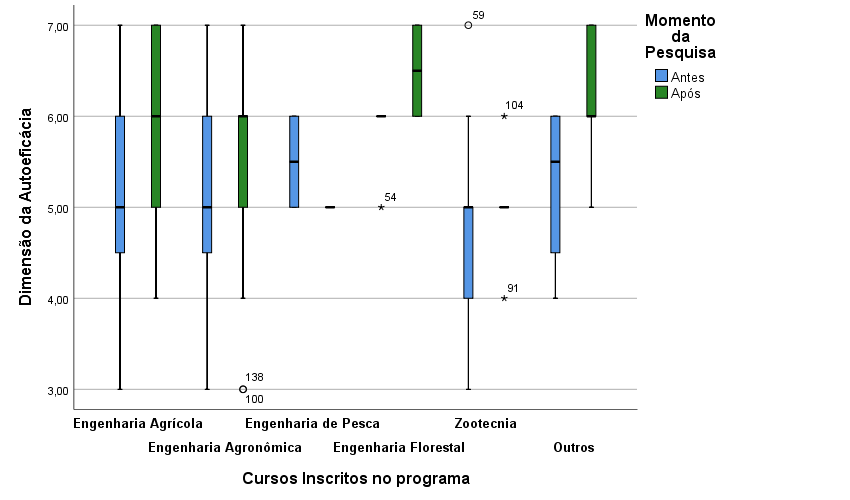
\includegraphics[scale=0.4]{Imagens/boxplot_autoeficacia.png}
\fonte{Autoria própria}
\label{figura_34}
\end{figure}


No Apêndice \ref{tab:amostras_autoeficacia} (Tabela \ref{tabela_5}), quando analisadas as questões individualmente, nota-se que as questões “Fazer análises financeiras”, “Reduzir riscos e incertezas”, “Assumir riscos calculados”, “Administrar o tempo estabelecendo metas” e “Conduzir minha própria empresa ao sucesso” obtiveram diferença significativa de 0,002, 0,003, 0,024, 0,018 e 0,028 respectivamente, tais valores foram menores que o intervalo de confiança que é de 0,05. Em outras palavras, houve elevada mudança para a autoeficácia dos alunos participantes nos quesitos relacionados diretamente ao plano de ensino do programa. Desta forma, o programa pode ter influenciado na melhoria da autoeficácia para análise financeira dos negócios (Lean Canvas), na predição de riscos e possíveis mitigações (Project Model Canvas), no gerenciamento ágil do tempo e atividades relacionadas à inovação (metodologias ágeis), e à promoção da disposição ao assumir riscos calculados em novos empreendimentos. Tais resultados se aproximam dos observados por \cite{schaefer_formacao_2017} que investigou as necessidades motivacionais que influenciam a intenção de potenciais empreendedores, e observou que a educação para o empreendedorismo no meio acadêmico promove melhorias da autoeficácia empreendedora.


O fato de o programa Empreenda Agro Sustentável ter um caráter de pré-aceleração, ele possuía o objetivo de suprir uma lacuna na formação dos discentes das ciências agrárias e demais áreas da Universidade Federal de Sergipe em relação ao desenvolvimento de um pensamento empreendedor, por meio da promoção de ciclos de oficinas, visando a disseminação dos valores e técnicas do gerenciamento ágil e a promoção do empreendedorismo capaz de aplicar tais metodologias na produção rural. 

Assim, o programa pode ter influenciado na melhoria da autoeficácia para análise financeira dos negócios, na predição de riscos e possíveis mitigações, no gerenciamento ágil do tempo e atividades relacionadas à inovação, e à promoção da disposição ao assumir riscos calculados em novos empreendimentos. Tais resultados se aproximam dos observados por \citeonline{schafer_be_2018} que investigou as necessidades motivacionais que influenciam a intenção de potenciais empreendedores, e observou que a educação para o empreendedorismo no meio acadêmico promove melhorias da autoeficácia empresarial. 

Foi observado também que a desejabilidade de criar negócios para o âmbito social pode ser determinada pela vontade dos alunos de autorrealização e autonomia pessoal após a vivência de conteúdos voltados à educação em empreendedorismo \cite{de_souza_qualidade_2017}.

Observando as demais perguntas e afirmações presentes na Tabela \ref{tabela_5}, é possível visualizar que, mesmo não apresentando diferença significativa, as afirmações “Estabelecer e atingir metas e objetivos”, “Gerar novas ideias” e “Começar minha própria empresa” mostram mudança positiva no valor do posto médio quando comparado ao antes e após: de 64,67 para 76,78, de 64,61 para 76,87 e de 64,96 para 76,35, respectivamente. Tais mudanças podem estar relacionadas à participação dos discentes neste tipo de programa, que pode os conduzir à expectativa de sucesso no desenvolvimento de novos negócios, assim como a confiabilidade de arriscar-se em negócios planejados \cite{nunes_associacoes_2011}. Desta forma, observando os dados obtidos nesta pesquisa, o Programa Empreenda Agro Sustentável proporcionou uma mobilização positiva sobre a autoeficácia dos participantes.

Neste sentido, considerando os resultados da dimensão autoeficácia observada no estudo, não se rejeita a hipótese nula (H₀) (Não há diferença entre as médias das medidas que averiguam o perfil empreendedor entre os alunos participantes do Programa de extensão Empreenda Agro Sustentável), quando observado os resultados da diferença apresentada no teste estatístico. Contudo, o programa Empreenda Agro Sustentável proporcionou uma mobilização positiva das respostas quando se comparado aos resultados iniciais dos participantes.


\subsection{Dimensão da Participação Familiar e Influência de Terceiros no Desenvolvimento do Empreendedorismo}

É de suma importância a análise sobre a influência da família e contatos próximos ao estudante propenso a empreender, já que a família é uma importante fonte de \textit{networking} para novos negócios \cite{soto_does_2019,raza_influence_2019,kupp_when_2019}, desde o financiamento no estágio inicial do negócio \cite{soto_does_2019,edelman_impact_2016} até os cuidados no âmbito familiar \cite{meliou_family_2020}  \cite{puzi_transgenerational_2020}. Pesquisas atuais sugerem que o potencial transformacional dos cuidados familiares pode influenciar positivamente para a viabilidade dos negócios e posiciona a família em um ponto-chave para o surgimento de novos negócios \cite{georgescu_impact_2020,jena_measuring_2020,porfirio_family_2020}. No entanto, o programa não influenciou na dimensão da participação familiar dos alunos vinculados ao programa (Figura \ref{figura_60}). Os dados apresentados demonstram que esta dimensão deve ser melhor explorada em futuras pesquisas, visto que esta dimensão pode influenciar negativamente na escalabilidade do negócio planejado pelo novo empreendedor. Os resultados podem ser observados no Apêndice \ref{tab:amostras_familiar} e Tabela \ref{tabela_familair}.


\begin{figure}[H]
\centering
\caption{\textbf{Contagem geral por momento da pesquisa sobre a participação familiar e influência de terceiros}}
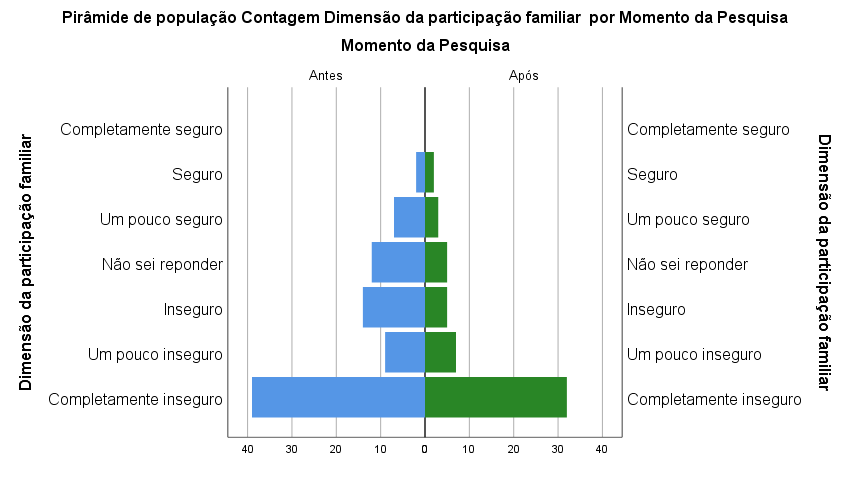
\includegraphics[scale=0.4]{Imagens/dimensao_familiar.png}
\fonte{O autor}
\label{figura_60}
\end{figure}

A família a costuma desempenhar importantes funções de incubação no processo de criação de novos empreendimentos, uma vez que muitos negócios podem surgir do empreendedorismo transgeracional \cite{puzi_transgenerational_2020,meliou_family_2020}, ou da mobilização de recursos familiares, demonstrando a importância desta dimensão ser melhor estudada em futuros trabalhos. 

Quando observado o gráfico Box Plot sobre a intenção empreendedora separados por cursos (Figura \ref{boxplotfamilia}), o curso de Engenharia Agrícola demonstrou mobilidade positiva no 2º e 3º quartis saindo da afirmação “Concordo em partes” (5,00) para a afirmação “Concordo completamente” (7,00), assim como uma redução na dispersão na frequência das respostas.  



\begin{figure}[H]
\centering
\caption{\textbf{Box plot  por momento da pesquisa sobre a participação familiar e influência de terceiros}}
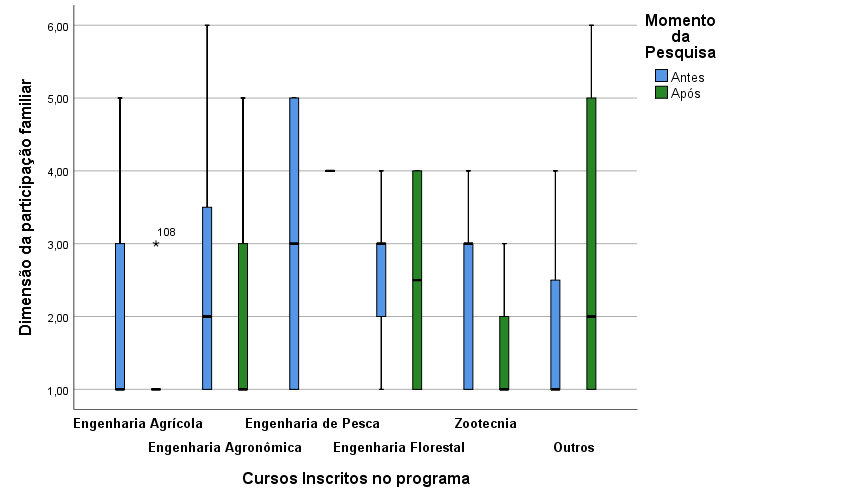
\includegraphics[scale=0.4]{Imagens/boxplot_familia.png}
\fonte{O autor}
\label{boxplotfamilia}
\end{figure}


Para o curso de engenharia Agronômica não houve mudança no 2º quartil, no entanto foi observado que a dispersão dos resultados aumentou à medida que o programa evoluiu, demostrando que mesmo não havendo mobilidade do segundo quartil, o quarto quartil aumentou significativamente os valores, um provável motivo foi a melhoria da intenção em empreender posteriormente ao programa. Foi observado apenas um outlier, o participante 116.

O curso de Engenharia de pesca apresentou uma ligeira redução dos resultados, um provável fator foi a pouca participação dos alunos deste curso no programa Empreenda Agro Sustentável, reduzindo assim o grau de liberdade dos dados obtidos. 

O curso de Zootecnia apresentou uma diferença positiva quando observados os valores localizados no 2º quartil, no momento anterior ao programa a frequência das afirmações estavam entre o \textit{Concordo em partes} (5,00) e \textit{Concordo} (6,00), passando a estar localizado entre a afirmação \textit{Concordo} (6,00) e \textit{Concordo plenamente} (7,00). Houve uma redução da dispersão dos dados observados após o programa, destacando apenas um outlier, o participante 131. Já nos demais cursos que participaram da pesquisa, foi observada uma mobilidade positiva do 2º quartil (mediana), saindo de \textit{Concordo em partes} (5,00) para \textit{Concordo completamente} (7,00).

Observando as questões relacionadas com as satisfações pessoais e profissionais dos discentes (Apêndice \ref{tab:amostras_familiar}), é possível verificar que as afirmações: \textit{Ser empreendedor me traria grande satisfação} e \textit{Uma carreira de empreendedor é atrativa para mim} apresentaram mudanças positivas no questionário analisado. Tais questões relacionadas à intenção empreendedora demonstram também que a participação constante em métodos educacionais que promovam o desenvolvimento da intenção empreendedora e autoeficácia nos participantes, interfere positivamente na autoconfiança e melhoria na satisfação profissional e pessoal, já que ambas estão associadas \cite{nassar_junior_fatores_2016}.

Estes fatores (satisfação pessoal e profissional) são de suma importância ao profissional que busca iniciar um novo negócio ou trabalhar com inovação, pois os fracassos em determinados projetos ao longo de sua carreira podem ser uma constante, e saber lidar com estes entraves deve ser uma habilidade adquirida ao longo do tempo \cite{edelman_impact_2016}.

O estudo observou que para a questão \textit{Eu já sou patrão na empresa que criei}, obteve-se desempenho negativo, provavelmente pela ocorrência de evasão dos alunos ao longo dos workshops realizados no programa, que foi demonstrado por defasagem nas respostas, de maneira que podemos inferir que permaneceram apenas os alunos que não são donos de negócios. A afirmação \textit{Se tivesse oportunidade e os recursos eu me tornaria um empreendedor}, apresentou diferença significativa positiva. 

A Intenção Empreendedora antecede o passo de criação do negócio, assim esta questão traz como certo que as restrições financeiras, falta de informação e a insegurança em capital específico podem interferir na abertura de novos negócios mesmo que esteja presente a Intenção Empreendedora \cite{auguste_what_2016}.

Quando observado o posto médio da questão “Por gentileza, indique se você tem pensado e o quão seriamente tem pensado em criar seu próprio negócio” houve uma ligeira mudança positiva que foi de 64,34 para 76,17. 

Esta questão está ligada ao fato de que a vivência constante do aluno em um ambiente que proporciona conteúdos e conhecimentos relacionados ao empreendedorismo e inovação, pode influenciar este a pensar e planejar o desenvolvimento de novos negócios, demonstrando uma real necessidade do surgimento de programas que incentivem ao desenvolvimento de novos negócios, cabendo aos locais de ensino proporcionar ao máximo essas vivências \cite{damanpour_phases_2006}.

A intenção em gerar um novo negócio tal qual a aqui discutida, é considerado um dos melhores preditores do empreendedorismo bem sucedido \cite{ajzen_attitudes_1987,garcia-rodriguez_entrepreneurial_2017,krueger_potencial_2018}, e é capaz de modificar positivamente não somente o novo empreendedor, mas também seu meio social como um todo, gerando emprego e renda direta e indiretamente \cite{gonzaga_infraestrutura_2017}.



\subsection{Dimensão e Intenção ao Empreendedorismo dos Estudantes}

Para impulsionar as atividades empreendedoras dos alunos, é essencial identificar os fatores que formam as intenções empreendedoras e investigar como o desenvolvimento desses fatores pode ser influenciado por programas educacionais \cite{gubik_entrepreneurial_2019}. 


A dimensão da intenção empreendedora tem como base a Teoria da Ação Planificada (TAP), que é amplamente utilizada para prever diferentes tipos de intensões comportamentais em diferentes áreas de estudo \cite{oliveira_educacao_2016,ros_psicologisocial_2001}. 

Por meio da análise desta dimensão, é possível  compreender e predizer não só a partir de fatores psicológicos, como vontade e segurança, mas também fatores sociais, como a interação indivíduo e sociedade (Krueger et al., 2000). Assim, por meio desta dimensão é possível observar o quão um modelo de ensino pode influenciar positivamente ou negativamente os participantes.

É possível observar no Histograma (Figura \ref{figura_45}) que ao participar de um programa educacional que promova atividades cadenciadas para o empreendedorismo, os alunos modificaram positivamente a sua intenção em empreender, passando de “Não sei responder” e “Concordo em partes” para “Concordo em partes” e “Concordo completamente”. Demostrando que a aplicação de ações motivacionais e processos educacionais com metodologias ativas  com incentivo ao empreendedorismo pode ser uma efetiva ferramenta para a melhoria da intenção em empreender \cite{fayolle_beyond_2014}. É possível observar também que as respostas “Discordo completamente” e “Discordo em parte” se anularam à medida que o programa se desenvolveu, corroborando a afirmação anteriormente dita, que o programa influenciou positivamente os alunos participantes.


\begin{figure}[H]
\centering
\caption{\textbf{Contagem geral por momento da pesquisa sobre a dimensão Intenção Empreendedora}}
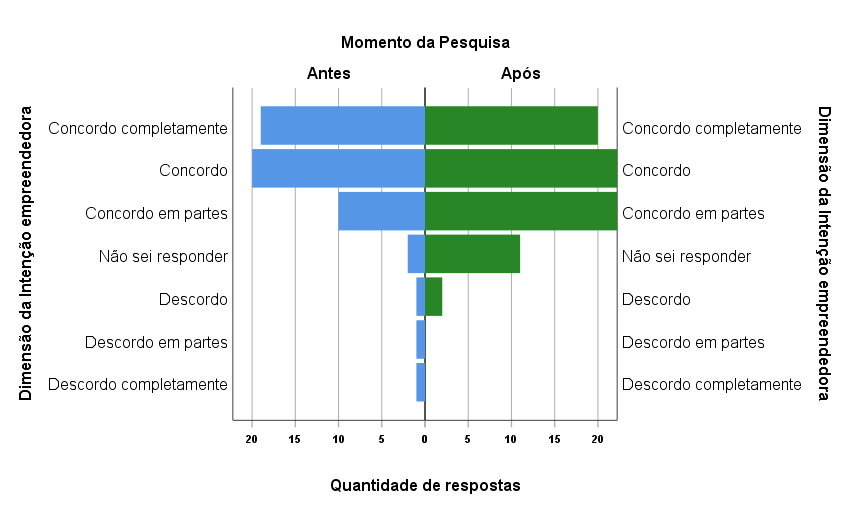
\includegraphics[scale=0.4]{Imagens/dimensao_empreendedora.png}
\fonte{O autor}
\label{figura_45}
\end{figure}


A ação de empreender como uma rotina ocorre ao longo do tempo, começa muito antes do momento em que um indivíduo cria um negócio. Assim, como em todos os comportamentos, é necessário um processo de planejamento para atingir o estágio de Intenção ao empreendedorismo, cabendo aos centros de ensino a promoção contínua e imersão frequente aos conteúdos relacionados \cite{garcia-rodriguez_entrepreneurial_2017}.

Quando analisado o resultado das respostas para as questões presente na Tabela \ref{tabela_6} apresentada no Apêndice \ref{tab:amostras_intencao_empreendedora}, mostra que ao participar de um programa educacional que promova atividades cadenciadas para o empreendedorismo, a intenção de empreender pode ser influenciada positivamente. Desta forma, a aplicação de teorias motivacionais e de processos educacionais ativos buscando o incentivo ao empreendedorismo pode ser aceita na medida que seja tida como frequente a vivência destes conteúdos e práticas \cite{fayolle_beyond_2014}.

As questões: \textbf{"Ser empreendedor me traria grande satisfação"} e \textbf{"Uma carreira de empreendedor é atrativa para mim"} (Apêndice \ref{tab:amostras_intencao_empreendedora}, Tabela \ref{tabela_6}) apesentaram mudanças positivas no questionário analisado. Tais questões relacionadas à intenção empreendedora demostram que a melhoria da autoeficácia promoveu maior segurança aos participantes, influenciando diretamente na intenção empreendedora. \citeonline{adelaja_students_2018} afirmam que a educação em empreendedorismo pode fornecer aos indivíduos o conhecimento específico necessário para o desempenho das tarefas e a solução de novos problemas. São fatores de suma importância ao empreendedorismo, mas para que surjam resultados satisfatórios, apenas a aplicação da educação em empreendedorismo não representa sucesso, de maneira que há necessidade de interações multidisciplinaridade dos conteúdos e do apoio familiar \cite{edelman_impact_2016}. 

A segurança financeira e o interesse pessoal são também importantes fatores, por isso é significativo o somatório de todas dimensões. No entanto, as intenções pessoais são influenciadas pelos processos de socialização, portanto, são parcialmente determinadas pelos valores culturais predominantes na sociedade \cite{schwartz_les_2006}, podendo esta, sozinha, não ser suficiente para mudar o comportamento dos alunos \cite{adelaja_students_2018}. Desta forma, a educação em empreendedorismo quando direcionada à melhoria da intenção empreendedora, deve ser uma prática comum e melhor vivenciada em ambiente real \cite{damanpour_phases_2006}, cabendo aos locais de ensino proporcionar ao máximo essas vivências. Essa intenção, portanto, surge anteriormente à criação de um empreendimento e pode ser considerada um dos melhores preditores do empreendedorismo bem-sucedido \cite{ajzen_attitudes_1987,krueger_competing_2000,garcia-rodriguez_entrepreneurial_2017}.

O papel da educação no empreendedorismo atualmente é o tópico mais investigado na literatura empresarial, visto  que a educação focada na promoção do empreendedorismo, influencia os alunos a adquirirem o conhecimento necessário para administrar um negócio e, assim,  desenvolver sua aptidão empreendedora \cite{nowinski_impact_2019}. Consequentemente, há melhoria na autoeficácia \cite{egerova_does_2017} aumentando a escalabilidade para novos negócios e as chances de sucesso \cite{kolstad_education_2015}.

A Intenção Empreendedora é uma das características do nível individual e dos contextos acadêmicos e sociais, com algum grau de efeitos específicos durante a vida acadêmica. Desta forma, diversificar os conteúdos dos futuros profissionais é uma questão crítica que merece atenção da comunidade de ensino de engenharia \cite{gilmartin_entrepreneurial_2019}.

O estudo observou que para a questão \textbf{"Eu já sou patrão na empresa que criei"} (Apêndice \ref{tab:amostras_intencao_empreendedora}, Tabela \ref{tabela_6}), obteve desempenho negativo, provavelmente pela ocorrência de evasão dos alunos ao longo dos workshops realizados no programa, que foi demonstrado por defasagem nas respostas, de maneira que podemos inferir que permaneceram apenas os(as) alunos(as) que não são donos(as) de negócios. 

A questão \textbf{"Se tivesse oportunidade e os recursos eu me tornaria um empreendedor"} (Apêndice \ref{tab:amostras_intencao_empreendedora}), apresentou diferença significativa positiva. A Intenção Empreendedora antecede o passo de criação do negócio, assim fatores como restrições financeiras, falta de informação e a incapacidade de acumular capital específico, podem interferir na abertura de novos negócios mesmo que esteja presente a Intenção Empreendedora \cite{auguste_what_2016}.

Quando observado o gráfico Box Plot sobre a intenção empreendedora separados por cursos (Figura \ref{figura_boxplot_intencao}), o curso de Engenharia Agrícola demonstrou mobilidade positiva no 2º e 3º quartis saindo da afirmação “Concordo em partes” (5,00) para a afirmação “Concordo completamente” (7,00), assim como uma redução na dispersão na frequência das respostas.


\begin{figure}[H]
\centering
\caption{\textbf{Box Splot com Resultado da dimensão da intenção empreendedora por curso}}
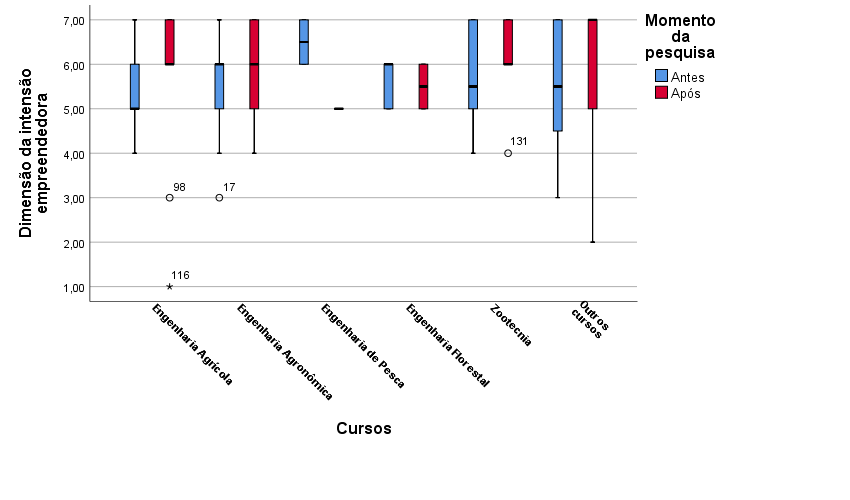
\includegraphics[scale=0.7]{Imagens/boxplot_intencao_empreendedora.png}
\fonte{O autor}
\label{figura_boxplot_intencao}
\end{figure}


Para o curso de engenharia Agronômica não houve mudança no 2º quartil, no entanto foi observado que a dispersão dos resultados aumentou à medida que o programa evoluiu, demostrando que mesmo não havendo mobilidade do segundo quartil, o quarto quartil aumentou significativamente os valores, um provável motivo foi a melhoria da intenção em empreender posteriormente ao programa. Foi observado apenas um outlier, o participante 116.

O curso de Engenharia de pesca apresentou uma ligeira redução dos resultados, um provável fator foi a pouca participação dos alunos deste curso no programa Empreenda Agro Sustentável, reduzindo assim o grau de liberdade dos dados obtidos.  

O curso de Zootecnia apresentou uma diferença positiva quando observados os valores localizados no 2º quartil, no momento anterior ao programa a frequência das afirmações estavam entre o \textbf{“Concordo em partes”} (5,00) e \textbf{“Concordo”} (6,00), passando a estar localizado entre a afirmação \textbf{“Concordo”} (6,00) e \textbf{“Concordo plenamente”} (7,00). Houve uma redução da dispersão dos dados observados após o programa, destacando apenas um outlier, o participante 131. 

Já nos demais cursos que participaram da pesquisa, foi observada uma mobilidade positiva do 2º quartil (mediana), saindo de “Concordo em partes” (5,00) para \textbf{“Concordo completamente”} (7,00).


%  \section{Contextualizando o Cenário da Prática}

%  \subsection{Realização do Primeiro Workshop}

% As atividades foram iniciadas com a abertura do programa que foi realizada pela equipe organizadora nos dias 9 e 10 de agosto de 2019, oportunidade da qual foi apresentada a programação dos Workshops, denominada de “A Jornada” (Figura 1). Esse momento do programa (1º Workshop) teve como foco o desenvolvimento de palestras e oficinas que abordaram temas relacionados ao empreendedorismo, tais como: startups, empreendedorismo, comportamento empreendedor e cultura empreendedora, problemas (segmentação do mercado) segundo as ODS (Objetivos do Desenvolvimento Sustentável) e Agritechs na palestra “Tecnologias digitais e as oportunidades para o Agronegócio”. Tendo como base pedagógica as metodologias ativas, aconteceu a oficina sobre Lean Canvas com foco na proposta de valor (Figura \ref{figura_29_1} do Apêndice \ref{app:workshop_1}).

%  \subsection{Realização do Segundo Workshop}

% A segunda oficina de aprendizagem que ocorreu nos dias 30 e 31 de agosto de 2019 quando foram abordados temas como a busca de oportunidades como característica fundamental de um empreendedor, economia colaborativa “Coworking”, e os benefícios do espaço compartilhado. Esses foram temas transversais que contribuíram para suporte teórico das equipes (Figura \ref{figura_segundo_workshop}). De forma proativa foram aprofundados os conhecimentos sobre cada bloco do Lean Canvas (solução, canais, métricas-chave, vantagem competitiva, receitas, custos, e o fechamento da proposta de valor) (Figura \ref{figura_segundo_workshop}). Segundo \citeonline{corallo_dynamic_2019} usar a estrutura proposta na definição do modelo de negócios permite aos alunos que buscam futuras propostas de negócios identificar várias estratégias de marketing, canais e métricas chave dedicadas a cada categoria de cliente, demonstrando que este tipo de ferramenta permite ao aluno melhorar o aprendizado e as taxas de sucesso nos projetos e simulação de negócios trazendo com isso a inovação educacional e o empreendedorismo a esfera acadêmica \cite{kukreti_entrepreneurship_2019}.

%  \subsection{Realização do Terceiro Workshop (Hackathon)}

%  O terceiro Workshop foi realizado nos dias 18 e 19 de outubro de 2019. Esse workshop foi conduzido no formato de Hackathon quando foi trabalhada a percepção do mercado, assim como a construção de protótipos como “Storyboard” e “Storytelling” (Figura \ref{figura_51}). Na educação empreendedora para o campo, o diálogo se mostra essencial quando é necessário a demonstração de um novo componente negocial visto que o ramo do agronegócio e essencialmente tradicional e requer formas atuais de apresentação quando se busca implementar novos métodos, processos e equipamentos, sendo assim os métodos de demonstração baseado em histórias se mostra bastante efetivos. 

% O Storyboard e o Storytelling como ferramentas de expressão para negócios, apresentam-se como formas de apresentações  didáticas de produtos por meio de narrativas construídas em prol de um produto, já que uma  narrativa desenvolvida para um produto pode criar experiências compartilhadas por meio da combinação de tempo e espaço \cite{langellier_storytelling_2004}. Desta forma a participação no desenvolvimento desta ferramenta os alunos participantes do programa ao desenvolver seus protótipos utilizando esta ferramenta, melhoram o senso de arranjo espacial dos produtos, a visão de marketing para o novo negócio \cite{brenes_improving_2019,brenes_improving_2019}, melhorou a capacidade de resolução de possíveis dúvidas que os clientes possam eventualmente ter e também aprenderam como otimizar o tempo de apresentação, tanto de forma compactada quanto expandida \cite{wahid_storyboard_2018,wu-rorrer_filling_2017}.

% Encontros como Hackathon consistiu em uma maratona de desenvolvimento e atividade prática, em que foi disponibilizado para as equipes a oportunidade de trabalhar suas ideias e construir um Mínimo Produto Viável (MVP) por meio da prototipagem, esta atividade promoveu a possibilidade de se trabalhar o projeto de forma multifuncional e permitiu que uma equipe reagisse de forma rápida e flexível as novas ideias surgidas diante do projeto de inovação e negócio, comportamento semelhante ao observado por \citeonline{zink_use_2017} em uma conferencia de inovação e engenharia. Além disso, três palestras de referências foram desenvolvidas durante essa fase possibilitando aos grupos um melhor desenvolvimento dos MVP:

%  \begin{itemize}
%   \item Oficina de Pitch para soluções inovadoras;
%   \item Hackathon Empreenda AGRO Sustentável e,
%   \item Marketing de relacionamento e marketing digital.
%  \end{itemize}

% A fase de teste não foi incluída neste workshop já que o momento final para tal demonstração foi articulado para o Demoday, no entanto, as equipes documentaram as soluções e os modelos de protótipos no intervalo entre o 3ª e 4ª oficina, para a apresentação final.

% \subsection{Realização do Quarto Workshop (Demoday)}


% O Demoday ou Dia de Demonstração (Figura \ref{figura_35}) dos modelos de negócios das sartups foi realizado no dia 22 de novembro de 2019. Esse foi o evento em que as startups (grupos de alunos) apresentaram seus produtos para os investidores, representados por ventures capitals, aceleradoras ou investidores-anjos.

% Nessa oportunidade, os jovens empreendedores apresentaram as ideias para comercialização diante da comunidade em geral que participou e possíveis investidores. Para alguns alunos foi a primeira chance participar de uma apresentação real em um evento de fora do ambiente universitário, momento também de oportunidade de novos networks e compartilhamento das ideias finais com os demais grupos.

% Na oportunidade foi desenvolvido uma pequena competição avaliada por quatro jurados das organizações parceiras e com base nos seguintes critérios: Possibilidade de negócio, adequação ao meio rural; nível de criatividade da inovação/negócio; desempenho na apresentação da equipe e documentação qualidade (MVP bem desenvolvido). 

\section{Inovações Desenvolvidas: Marcas e Produtos}
\label{inovacoes}

O programa foi concluído  com a formação e participação de 15 equipes, que foram nomeadas como segue por ordem alfabética: 

\begin{multicols}{3}
\centering
    \begin{itemize}
\item { Aqua plant;}
\item { Agrion;}
\item { AGROPEC;}
\item { Agro View;}
\item { BAgrotec;}
\item { Be Soluções;}
\item { Grão Nordestino;}
\item { Horta House;}
\item { Itecagro;}
\item { Impacto Pescados;}
\item { La Flora Pet;}
\item { MAMP;}
\item { Ranagro;}
\item { Tecno Coco;}
\item { Uneagro.}
\end{itemize}
\end{multicols}

O programa resultou um total de 16 marcas, 15 para os grupos e a marca própria do programa, como mostrado na Figura \ref{fig_marcas}.

Os modelos de negócios foram assim descritos (pitchs) pelas equipes:
\begin{figure}[H]
\centering
\caption{\textbf{Portfólio das marcas desenvolvidas durante o programa}}
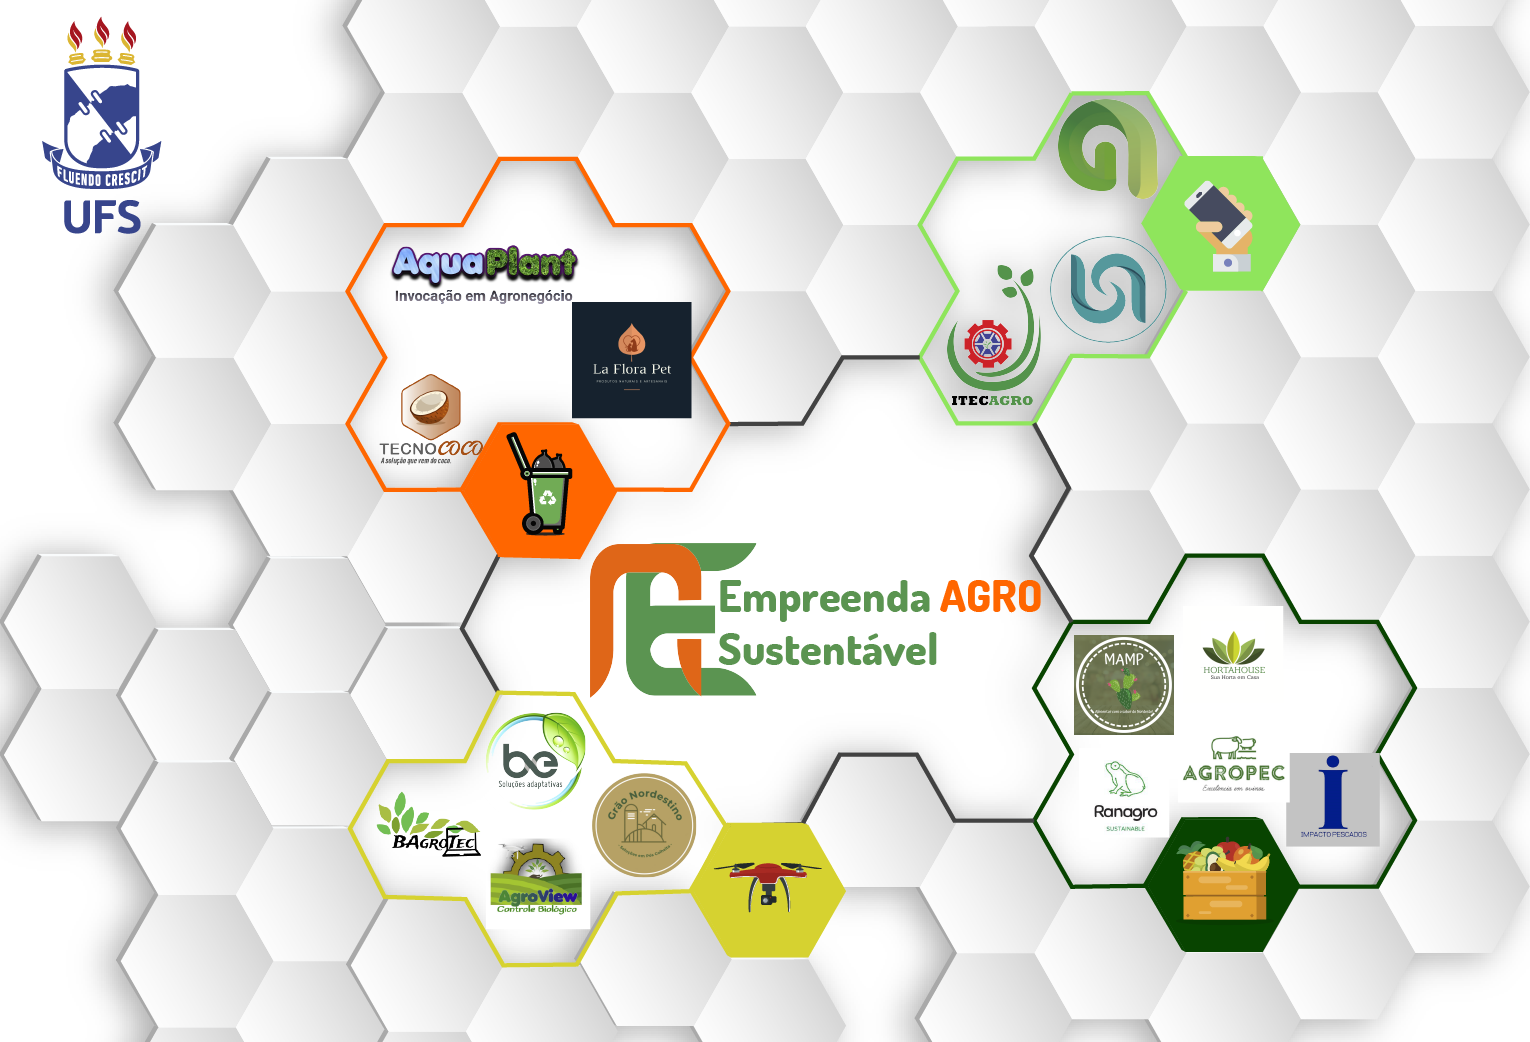
\includegraphics[scale=0.5]{Imagens/portfolio_2.png}
\fonte{O autor}
\label{fig_marcas}
\end{figure}


\subsection{Aqua Plant}

Startup que visa justamente acabar com as incertezas que afligem o agricultor quanto à sua produção, visto que o produto é um sistema de aquaponia fechado, com recirculação de água, ao qual no final do processo o produtor terá garantido proteína e hortaliças de qualidade.
O produto é integrado em pacotes de assistência técnica, tanto diretamente ao produtor como também em contratos com municípios.


\begin{figure}[H]
\centering
\caption{\textbf{Marca Aquaplant}}
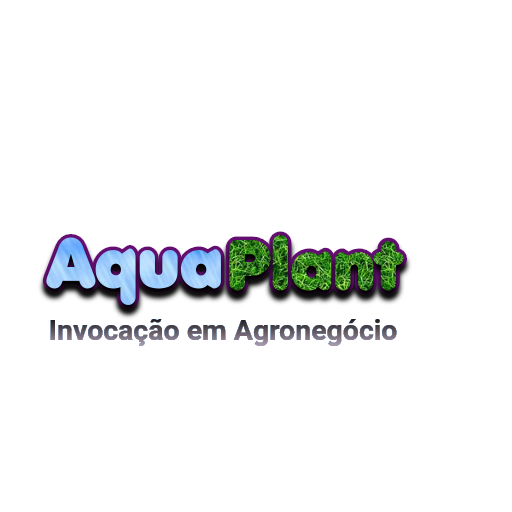
\includegraphics[scale=0.5]{Imagens/aquaplant.png}
\fonte{\cite{ufs_empreenda_2019}}
\label{figura_13}
\end{figure}


\subsection{Agrion}

Aplicativo desenvolvido por sistemas digitais, de modo a conectar diretamente os produtores aos mercados varejistas no processo de compra e venda de produtos agrícolas onde a lucratividade é prevista por meio da cobrança de taxação em cima do montante total de vendas, diferenciando valores de venda em atacado e varejo, e porcentagem por produto.


\begin{figure}[H]
\centering
\caption{\textbf{Marca Agrion}}

\includegraphics[scale=0.3]{Imagens/agrion.png}
\fonte{\cite{ufs_empreenda_2019}}
\label{figura_14}
\end{figure}

\subsection{BAgroTec}

O App TecAgro conecta o produtor ao profissional de agricultura, solucionando problemas no campo e consequentemente, gerando mercado de trabalho para os profissionais. Além do App, o site da BAgroTec irá auxiliar o cadastramento de produtores que apresentam dificuldades com a plataforma mobile. O aplicativo irá valorizar o profissional gerando currículo dentro da plataforma, possibilitando ao produtor ter acesso e retorno imediato do profissional. Esse aplicativo fornecerá dados que irá auxiliar ao profissional na tomada de decisão no campo.

\begin{figure}[H]
\centering
\caption{\textbf{Marca BAgroTec}}

\includegraphics[scale=1.5]{Imagens/bagrotec.png}
\fonte{\cite{ufs_empreenda_2019}}
\label{figura_15}
\end{figure}


\subsection{AGROPEC}


O modelo de negócio está baseado na produção de carne de cordeiro com eficiência zootécnica e no gerenciamento financeiro, além da bonificação dos resultados, compra e venda de produtos agrícolas onde a lucratividade é prevista por meio da cobrança de taxação em cima do montante total de vendas, diferenciando valores de venda em atacado e varejo, e porcentagem por produto.


\begin{figure}[H]
\centering
\caption{\textbf{Marca AGROPEC}}
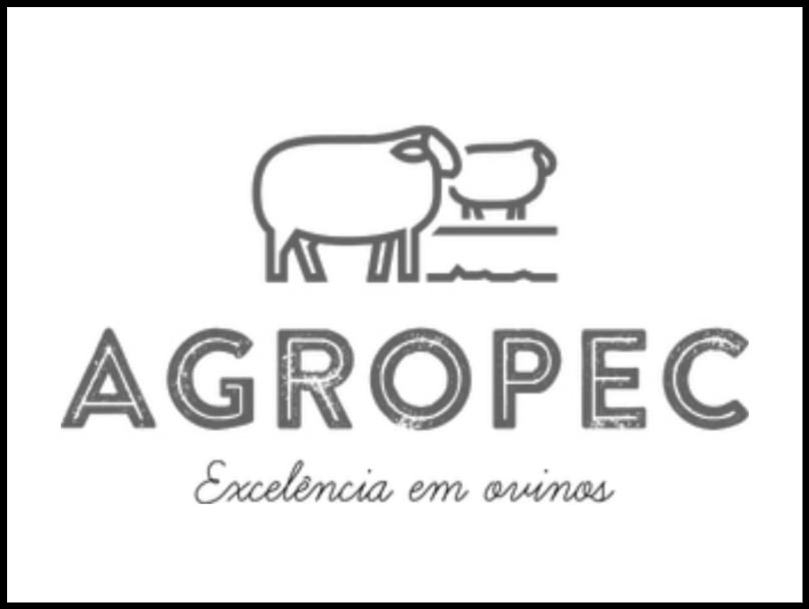
\includegraphics[scale=0.3]{Imagens/agropec.jpg}
\fonte{\cite{ufs_empreenda_2019}}
\label{figura_18}
\end{figure}

\subsection{Agro View}


Produto que monitora a produção. Para ser mais assertivo na identificação e tomada de decisão de aplicar os produtos na hora correta, os clientes terão que celebrarão um contrato mensal, havendo controle antes que as pragas possam causar danos severos e evitando uso desnecessário de agrotóxicos. 


\begin{figure}[!htb]
\centering
\caption{\textbf{Marca Agro View}}

\includegraphics[scale=0.2]{Imagens/agroview.jpg}
\fonte{\cite{ufs_empreenda_2019}}
\label{figura_19}
\end{figure}

\subsection{Be Soluções}

Para reduzir essa o desperdício de água, é proposto a utilização de um sistema diferente dos sistemas atuais, que possuem um alto custo e que não apresentam tantos recursos de forma unificada em um só equipamento. Foi desenvolvido um produto que proporciona uma alta precisão ao utilizar um sistema de dados coletados em tempo real, obtidos no local específico da cultura irrigada.

\begin{figure}[H]
\centering
\caption{\textbf{Marca Be Soluções}}
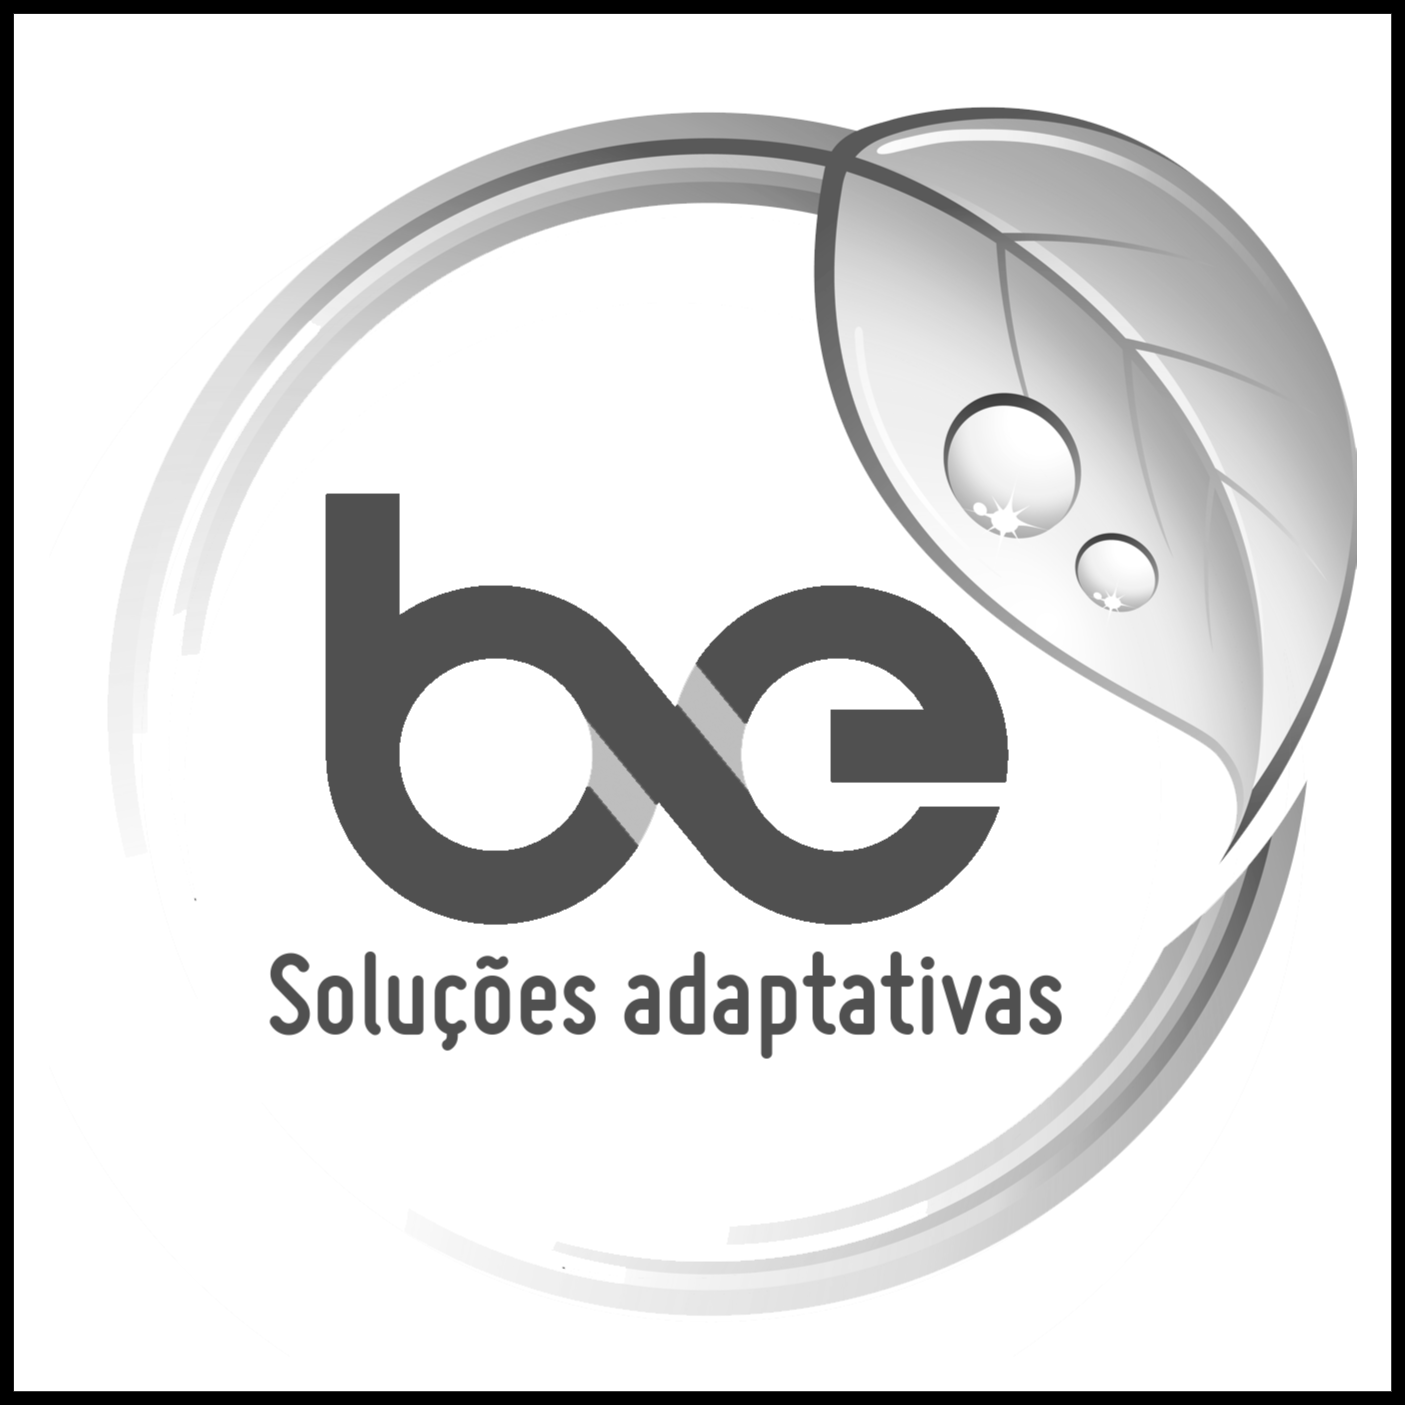
\includegraphics[scale=0.5]{Imagens/besolucoes.png}
\fonte{\cite{ufs_empreenda_2019}}
\label{figura_20}
\end{figure}

\subsection{Grão Nordestino}

Conhecendo a realidade do pequeno e médio produtor que por falta de uma unidade armazenadora perdem boa parte da sua colheita ou são obrigados a vender com o menor preço para que não venha a perder seu produto, a startup grão Nordestino produzirá silos de baixo custo e sustentáveis, agregando valor ao produto e combatendo o desperdício de alimentos mal armazenados.


\begin{figure}[H]
\centering
\caption{\textbf{Marca Grão Nordestino}}

\includegraphics[scale=0.4]{Imagens/graonordestino.png}
\fonte{\cite{ufs_empreenda_2019}}
\label{figura_21}
\end{figure}

\subsection{Horta House}


O número de empresas especializadas em consultoria para hortas urbanas ainda é insuficiente para atender essa demanda que continua a crescer. Tentando solucionar esse problema, muitas pessoas recorrem a ferramentas de busca na internet e acabam tomando como base instruções de pessoas que muitas vezes não possuem uma qualificação técnica adequada, o que em muitos casos não respondem adequadamente como desejado.


\begin{figure}[H]
\centering
\caption{\textbf{Marca Horta House}}

\includegraphics[scale=0.1]{Imagens/hortahouse.png}
\fonte{\cite{ufs_empreenda_2019}}
\label{figura_25}
\end{figure}

\subsection{ItecAgro}

A Plataforma visa uma interação direta com uma equipe multidisciplinar voltada para o agro, que se utiliza de sistemas digitais para dinamizar seu negócio de forma inovadora, empreendedora e sustentável. Vimos propor um canal facilitador, através de sistemas digitais para dinamizar o negócio da agricultura. A startup se propõe a desenvolver soluções através da assistência técnica de qualidade gerando valor ao produtor e promovendo responsabilidade socioambiental, e trabalho com excelência. Seguindo os valores de: inovação, humanização, sustentabilidade, ética, transparência, profissionalismo, confiabilidade e tecnologia.

\begin{figure}[!htb]
\centering
\caption{\textbf{Marca Itec Agro}}

\includegraphics[scale=0.15]{Imagens/itecagro.png}
\fonte{\cite{ufs_empreenda_2019}}
\label{figura_46}
\end{figure}
\newpage

\subsection{Impacto Pescados}

Startup especializada na criação de camarão do tipo Litopenaeus vannamei com a utilização de bomba movida a óleo diesel para sucção da água do mar viabilizando as trocas de água com uma maior frequência tornando o menor tempo de cultura, lançando no mercado um produto de qualidade com um menor período de cultivo. Podendo, assim, vender o produto a 15,0 0R\$ no mínimo. Além disso, existe o fato do preço elevado para o camarão. Sendo assim, soluciona-se esta problemática com criação de camarão em viveiros além de fazê-lo com o menor preço e melhor atendimento. 

\begin{figure}[H]
\centering
\caption{\textbf{Marca Impacto Pescados}}

\includegraphics[scale=0.4]{Imagens/impacto_pescados.jpg}
\fonte{\cite{ufs_empreenda_2019}}
\label{figura_23}
\end{figure}


\subsection{La Flora Pet}

Observando o crescimento do mercado PET nos últimos anos e a persistência nas dores sofridas pelos donos desses animais com relação a custo alto e acessibilidade a tratamentos eficientes, a La Flora Pet desenvolve produtos naturais e artesanais com base em extratos ou óleos essenciais cujo objetivo é prevenir. Após cadastramento de dados pessoais do cliente e usuário, a personalização consiste em escolher o extrato ou óleo essencial de acordo a finalidade terapêutica desejada, o formato, a cor e o tamanho do produto, constatadas essas informações será solicitado e após fabricação, o produto seguirá para o endereço do cliente.


\begin{figure}[H]
\centering
\caption{\textbf{Marca La Flora pet}}

\includegraphics[scale=5]{Imagens/laflorapet.png}
\fonte{\cite{ufs_empreenda_2019}}
\label{figura_24}
\end{figure}


\subsection{MAMP}

A palma não é um alimento convencional no Brasil, porém, no México e em outros países com influência mexicana já existem mais de 200 receitas utilizando essa espécie. O que torna o mercado muito amplo e com diversas oportunidades. Pensando nisso o produto foi desenvolvido principalmente para o público Fitness e vegetarianos. O mercado Fitness tem uma grande demanda por uma alimentação saudável, por isso trouxemos a Palma como alternativa para suprir essa carência do mercado, atualmente abastecido com produtos de alto custo, diferente do nosso produto de baixo custo e alto lucro.

\begin{figure}[H]
\centering
\caption{\textbf{Marca MAMP}}
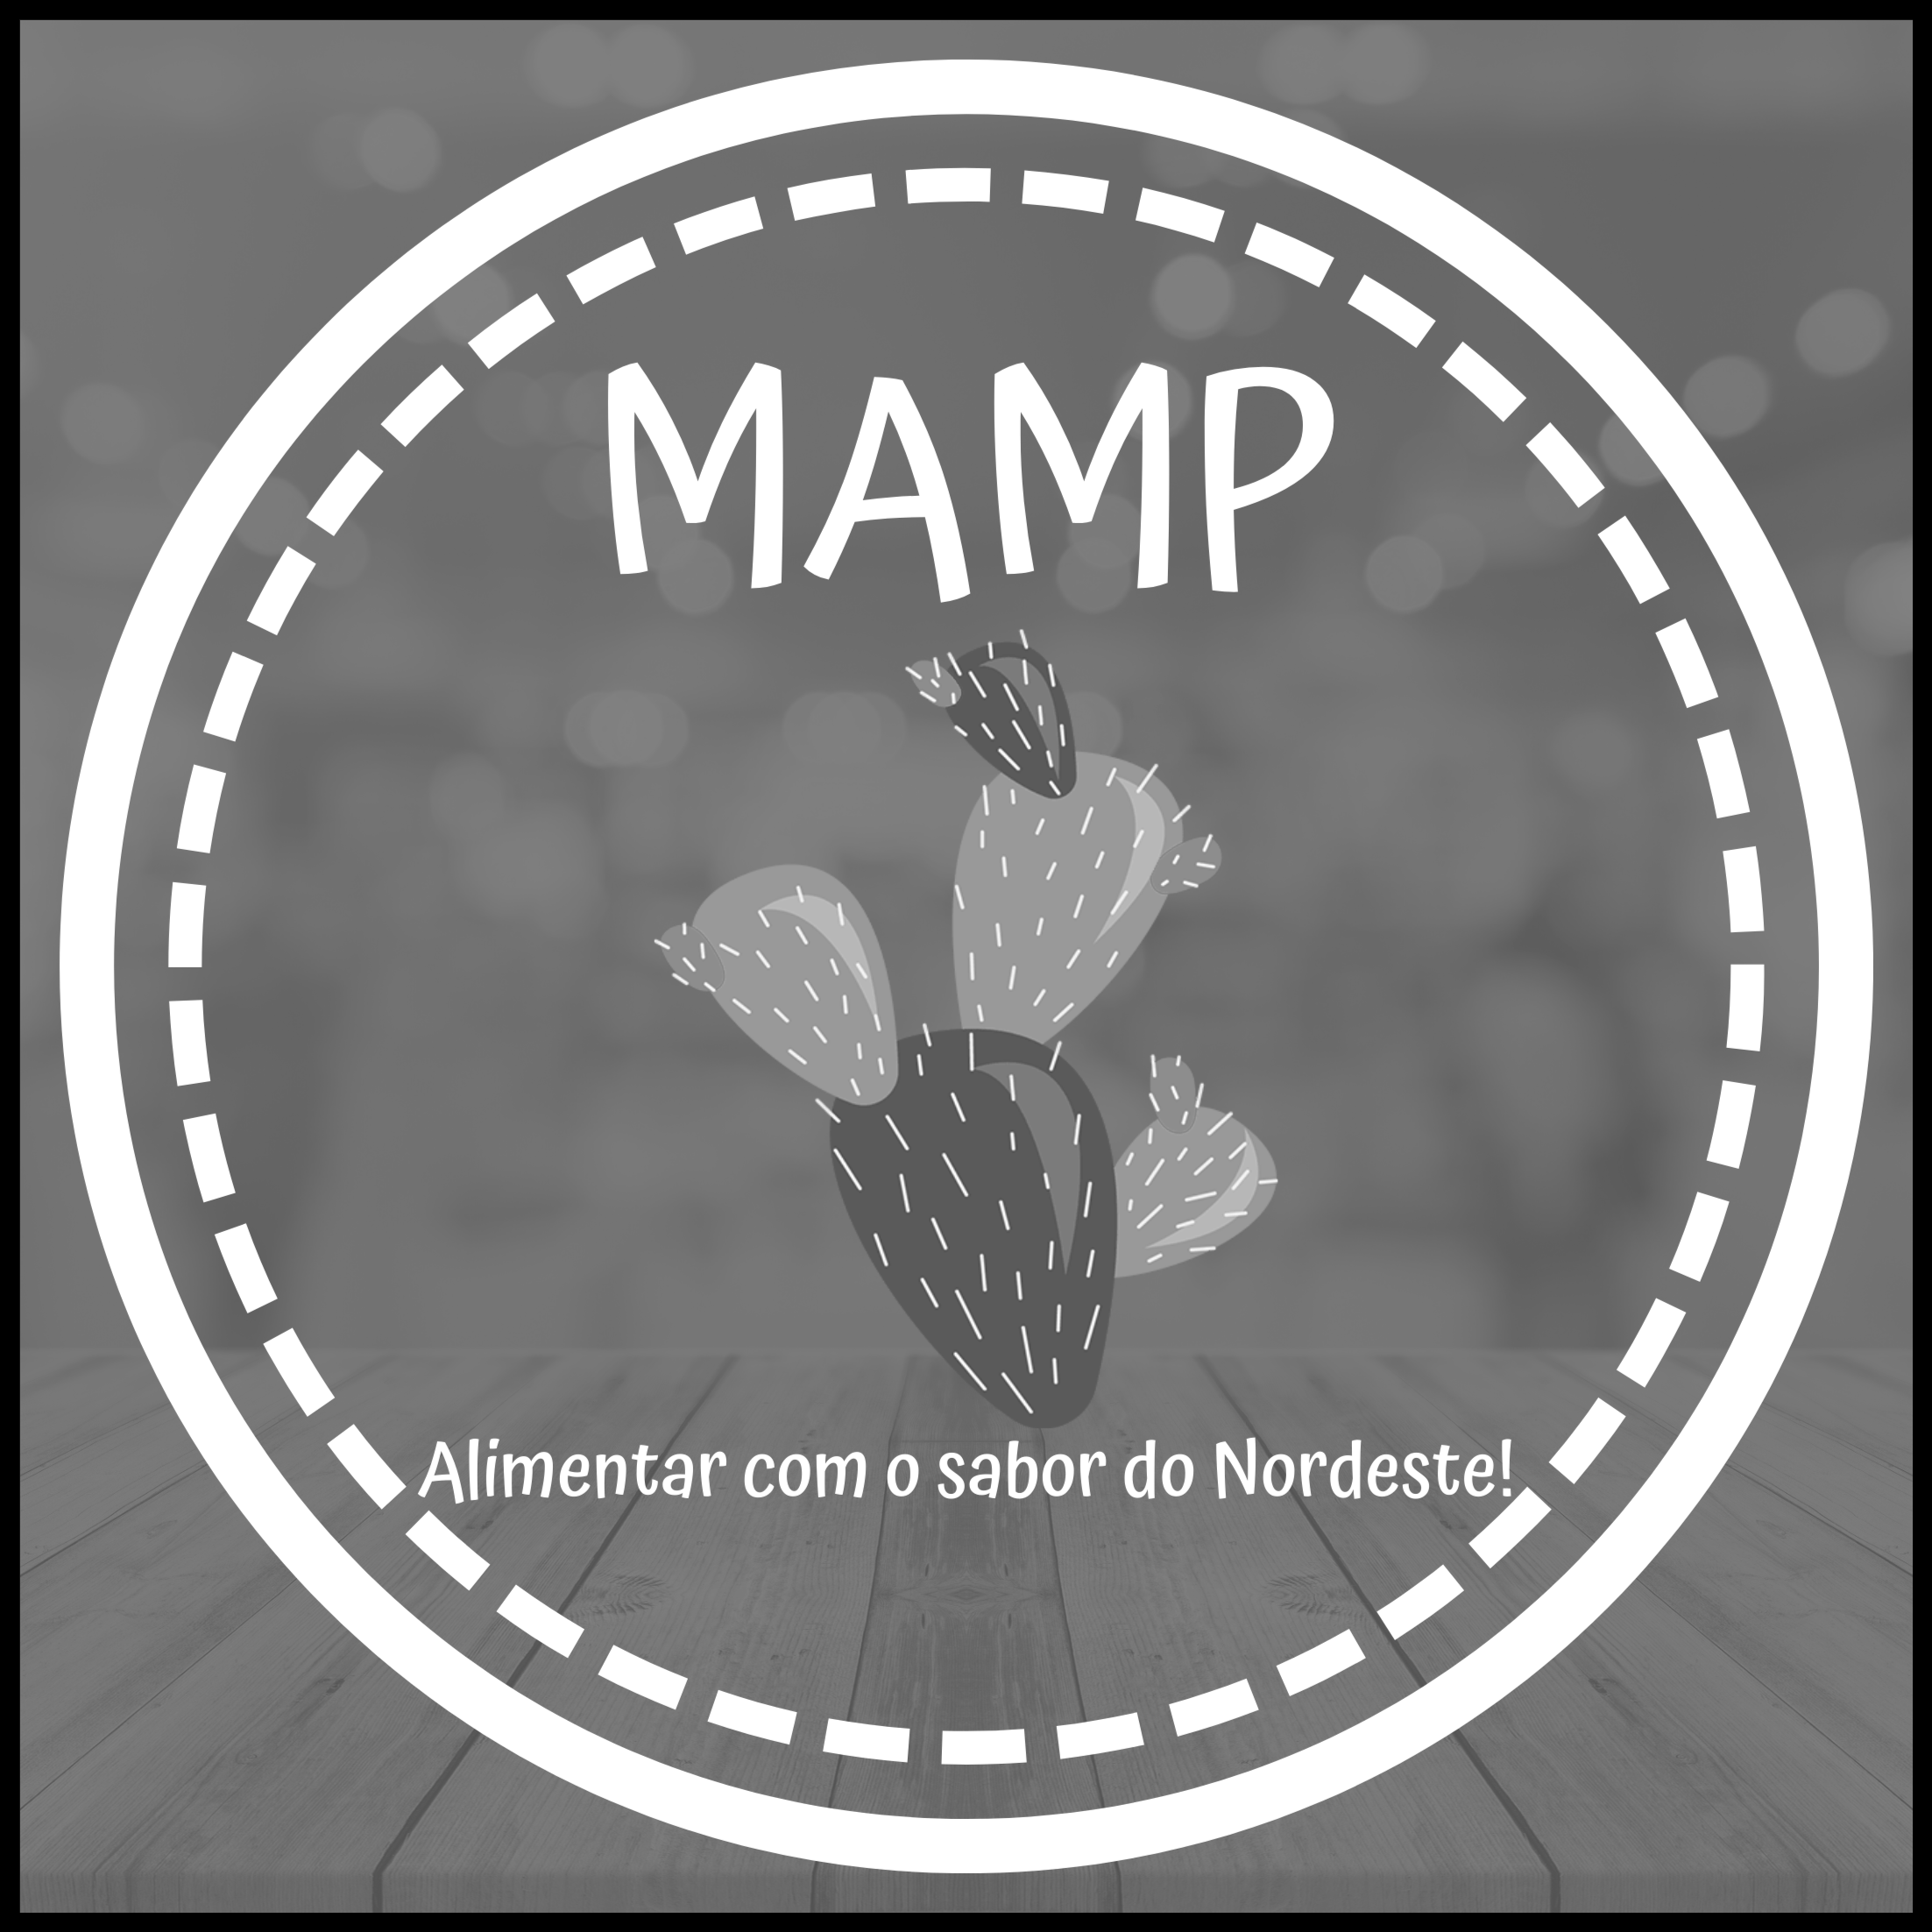
\includegraphics[scale=0.1]{Imagens/mamp.png}
\fonte{\cite{ufs_empreenda_2019}}
\label{figura_22}
\end{figure}


\subsection{Ranagro}

Com o mercado cada vez mais competitivo, se faz necessária uma inovação para alcançar o resultado satisfatório e economicamente viável para o produtor e consumidor, além de trazer tecnologias inovadoras para o ramo da ranicultura. A qualidade e sustentabilidade é vista como uma arma estratégica para a expansão da empresa. A ração oferecida no mercado é a mesma empregada na criação de peixes que acarreta um menor aproveitamento da carne e elevando o custo para a engorda. Assim a Ranagro, veio com uma proposta inovadora para o mercado que é a comercialização de uma ração específica, para haver menos custo, menor impacto ambiental, crescimento rápido, boa lucratividade e um alto aproveitamento. 



\begin{figure}[H]
\centering
\caption{\textbf{Marca Ranagro}}
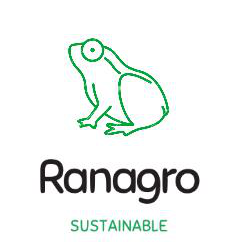
\includegraphics[scale=1]{Imagens/ranagro.png}
\fonte{\cite{ufs_empreenda_2019}}
\label{figura_26}
\end{figure}


\subsection{Marca Tecno Coco}

A ideia da Tecno Coco é gerar uma cadeia cíclica de produção onde o Campo produz o coco, que é destinado ao comerciante, vendido ao usuário onde é descartado e processada pela nossa Startup retornando ao Campo como insumo agrícola, auxiliando na produtividade. Outra parte será destinada a outras cadeias produtivas e manufaturadas, como material para isolamento acústico, reforço de materiais, enchimento de estofados, mantas para proteção do solo e muitos outros produtos que esse resíduo pode ser transformado. 

\begin{figure}[H]
\centering
\caption{\textbf{Tecno Coco}}

\includegraphics[scale=2]{Imagens/tecnococo.png}
\fonte{\cite{ufs_empreenda_2019}}
\label{tecno_coco}
\end{figure}


\subsection{Une Agro}

O aplicativo é desenvolvido tanto para o agricultor quanto para o distribuidor, pois, o distribuidor terá uma maior variedade de preços pelo mesmo produto. O aplicativo será totalmente gratuito, sendo que a receita da empresa se originará nas parcerias anunciantes e seus produtos no aplicativo, além de disponibilizar informações (produtos) para os usuários através de um pacote mensal ou anual, onde esses infoprodutos estarão relacionados ao próprio desenvolvimento de negócio dos usuários, como aulas e podcasts sobre gestão e produção agrícola. A marca pode ser vista na Figura \ref{figura_28})e os produtos podem ser vistos no Apêndice \ref{app:workshop_demoday}.

\begin{figure}[H]
\centering
\caption{\textbf{Marca Une Agro}}

\includegraphics[scale=1.5]{Imagens/uneagro.png}
\fonte{\cite{ufs_empreenda_2019}}
\label{figura_28}
\end{figure}




\subsection{Contribuição do Programa para inovação acadêmica}


Apesar do crescente interesse das pesquisas em inovação no meio acadêmico, isto é, o desenvolvimento de novos produtos oriundos das unidades de ensino, atualmente pouquíssimos estudos exploram como o meio acadêmico interfere no desenvolvimento de novos produtos direcionados ao meio rural de forma sustentável \cite{liu_new_2020}, já que os novos empreendimentos e startups são atores-chave na implementação de inovações direcionadas a uma produção agrícola menos impactante e mais sustentável \cite{fichter_impacts_2020}. Este estudo demonstra que a universidade com os programas de extensão universitária também pode ser um centro de pré-aceleração de novos negócios e  empreendimentos. 


\section{Materiais de Apoio para Desenvolvimento do Aprendizado Teórico dos Conteúdos: Aplicativo Empreenda Agro Sustentável}

Muitos aplicativos móveis agrícolas pagos e gratuitos foram desenvolvidos para o meio rural, abrangendo diversas áreas dentro e fora da propriedade rural \cite{silva_environment_2015}. A tecnologia da informação apresenta grandes potencialidades para auxiliar produtores rurais e profissionais da área na tomada de decisões estratégicas. Todavia, para o profissional das ciências agrárias tomar decisões assertivas, não basta apenas manusear a Tecnologia da Informação aplicada ao agronegócio, é necessário mudar a concepção dos processos a partir de sua informatização \cite{ferraz_tecnologia_2017}.

A área de Edtech no Brasil segue em franco crescimento. Segundo relatório da \citeonline{abstartups_mapeamento_2020} o país conta com 449 Startups focadas em aplicação sistemática de conhecimento científico para tarefas práticas, das quais 48,11/\% são direcionadas ao ensino superior, assim, o aplicativo Empreenda Agro se soma a estas ferramentas. Ele foi desenvolvido para ser ferramenta portátil, acessível e utilizável por acadêmicos das Ciências Agrárias no sentido de dar direcionamento educacional em empreendedorismo.

\subsection{Recursos e Funcionalidades do Aplicativo}

O aplicativo consiste em uma ‘interface’ com bancos de dados que permite ao usuário averiguar, de modo interativo, os conteúdos mais bem recomendados para o aprendizado da cultura empreendedora para as áreas das ciências agrárias. Ele foi desenvolvido seguindo o ‘design’ instrucional sistematizado, tais como a maioria dos aplicativos desenvolvidos para uso educacional observado por \citeonline{barra_metodos_2017}.

Para o acesso de dados através do dispositivo portátil, o mesmo pode ser instalado com apenas alguns cliques, onde o usuário não precisa estar inscrito ou participando do programa para efetuar o primeiro acesso. É necessário apenas ter disponibilidade de rede de Internet local ou móvel, que permita o primeiro acesso das informações. Após concluir a transmissão de dados para o aplicativo, não se faz necessário ter continuidade ao acesso de Internet para utilizar o aplicativo.


Durante a execução do aplicativo tem-se a tela de inicialização que apresenta a marca do aplicativo e do programa homônimo (Figura \ref{figura_42} \textcolor{blue}{(a)}). Após isto, tem início a tela principal do aplicativo (Figura \ref{figura_42} \textcolor{blue}{(b)}), que exibe uma lista de botões para selecionar o conteúdo de interesse do usuário e a forma de visualização. Estas funcionalidades podem ser acessadas por um menu lateral deslizante (Figura \ref{figura_42} \textcolor{blue}{(c)}), facilitando assim o manuseio do aplicativo pelo usuário final. 



\begin{figure}[H]
\FloatBarrier
\center
\caption{\textbf{Aplicativo Empreenda Agro Sustentável}}
\subfigure[ref1][Tela inicial]{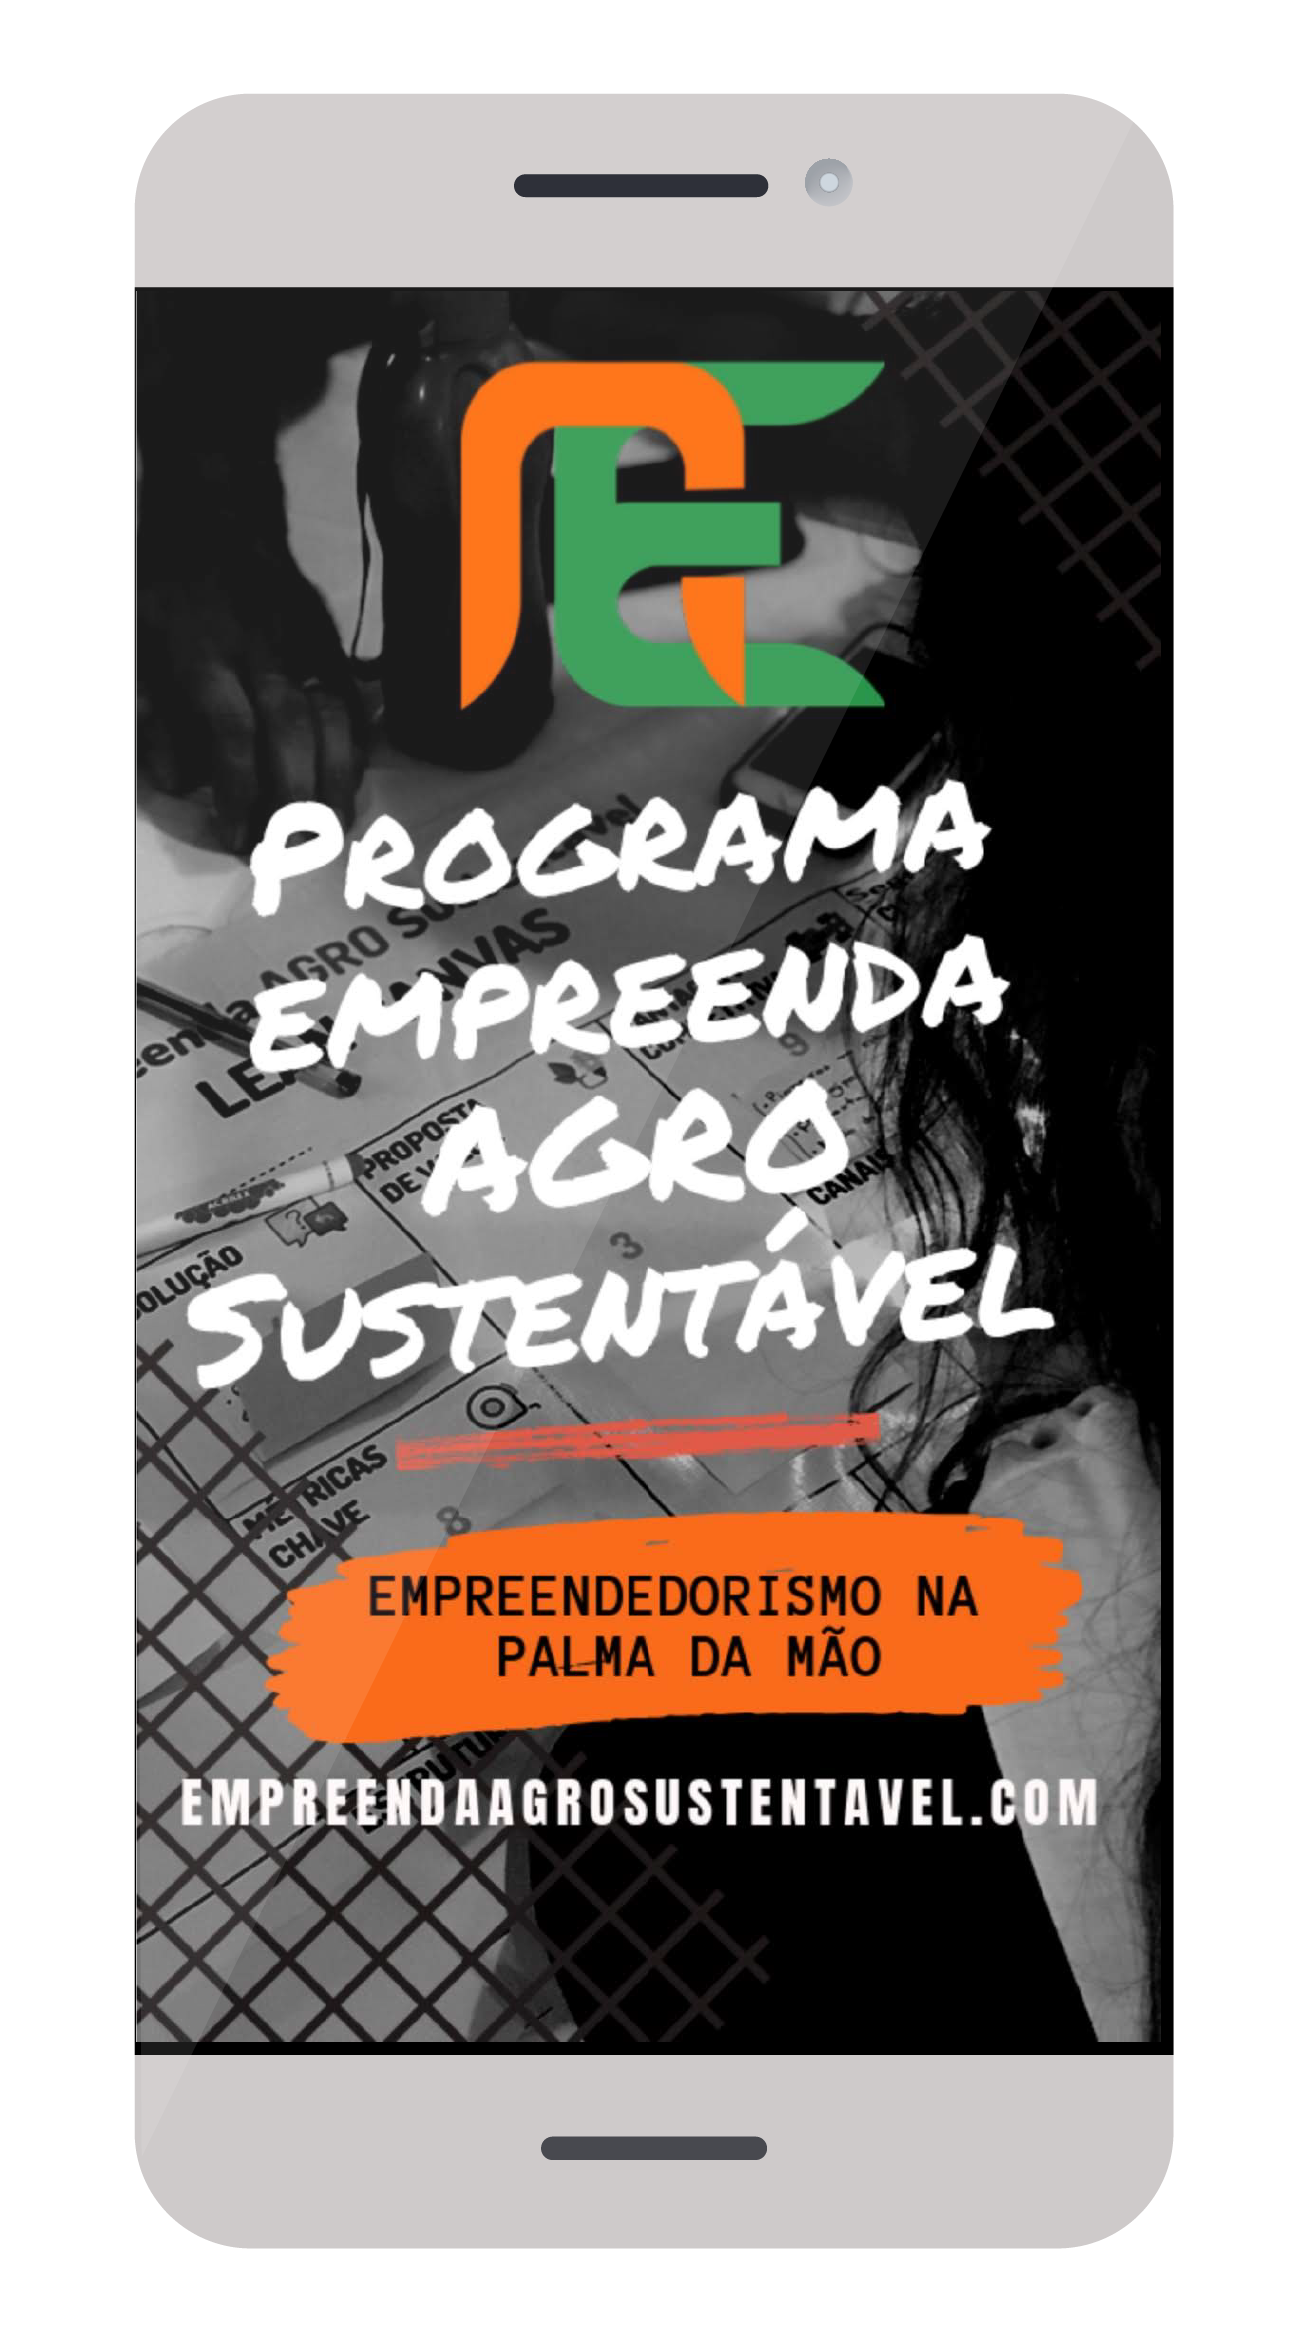
\includegraphics[scale=0.2]{Imagens/aplicativo_7.png}}
\qquad
\subfigure[ref2][Tela Principal]{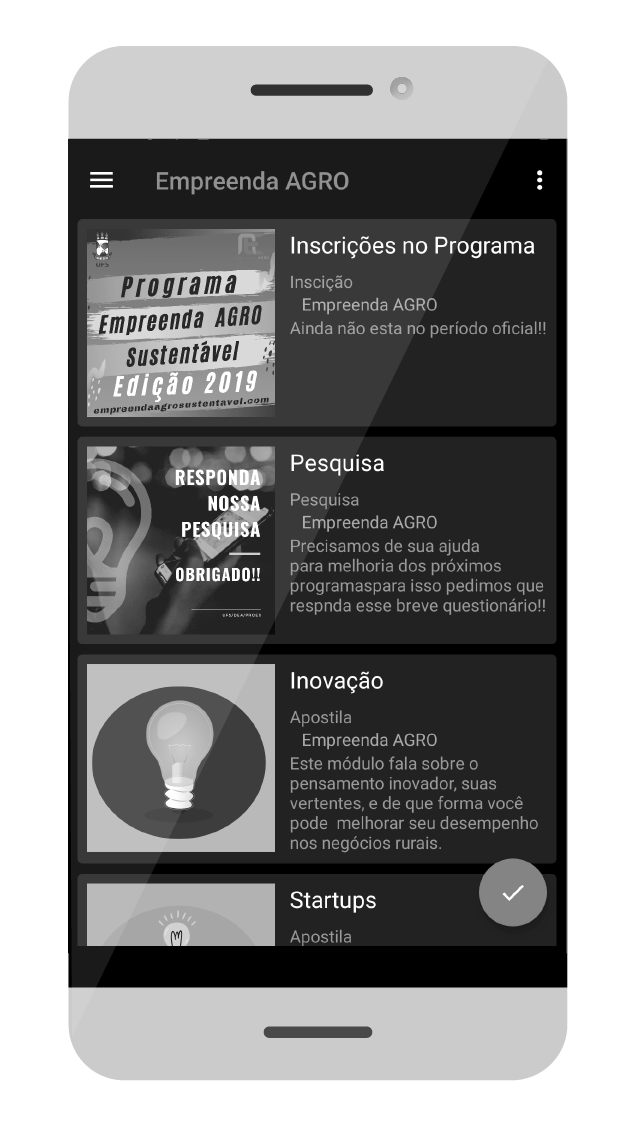
\includegraphics[scale=0.2]{Imagens/aplicativo_1.png}}
\qquad
\subfigure[ref3][\textit{Drawer list}]{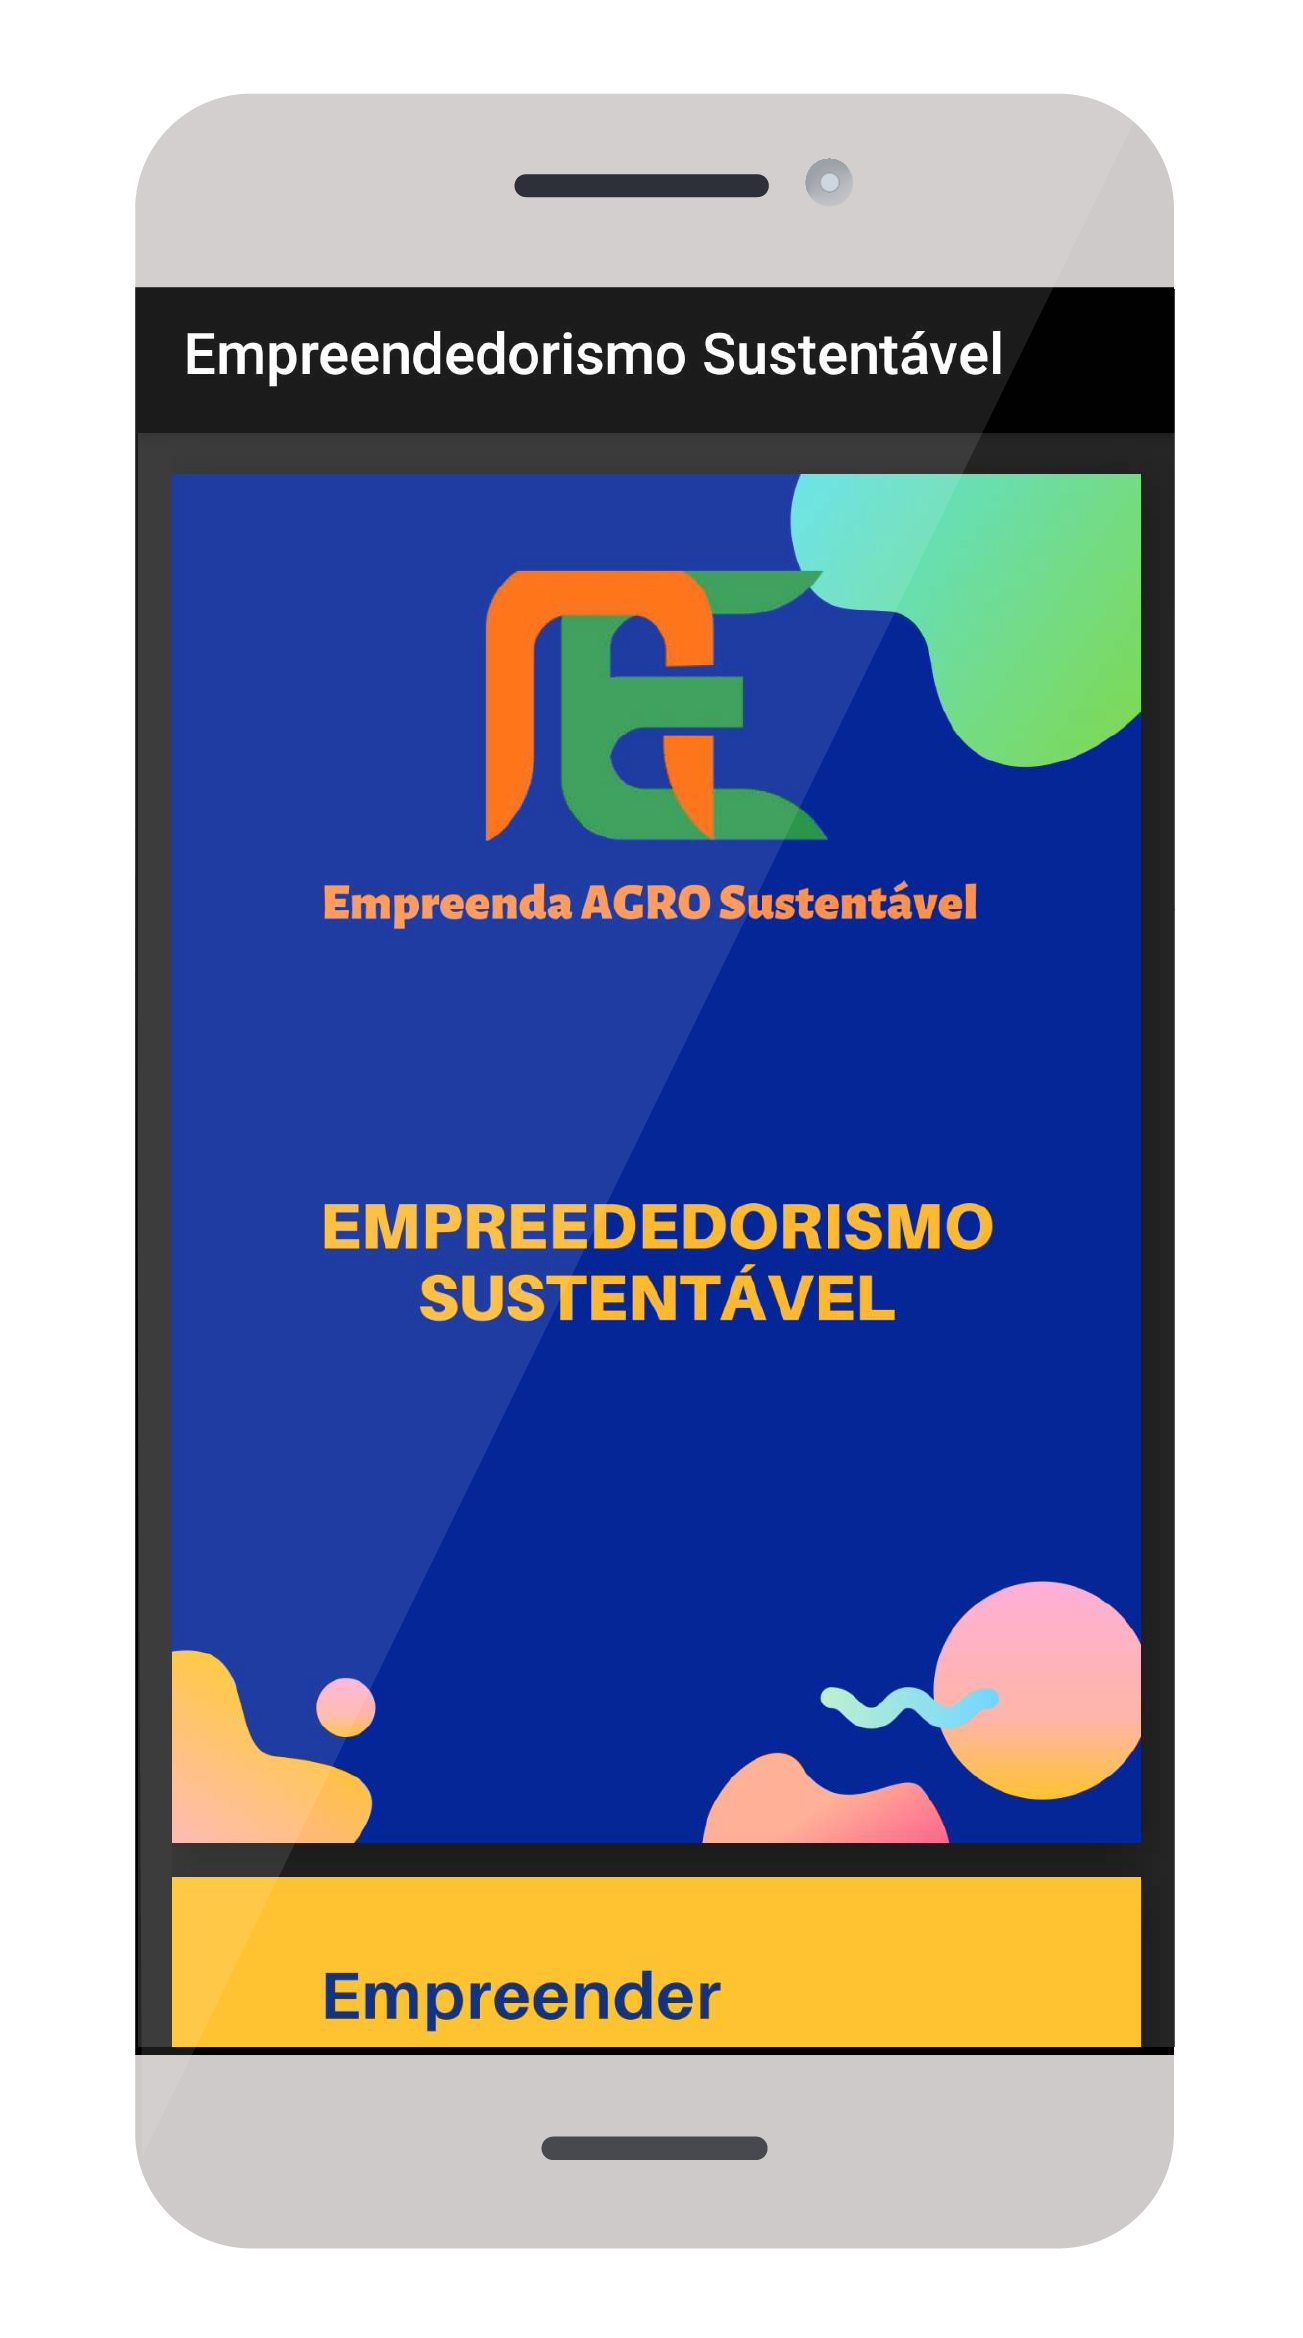
\includegraphics[scale=0.2]{Imagens/aplicativo_3.png}}
\fonte{O Autor}.
\label{figura_42}
\end{figure}
 

Os ‘podcasts’ gravados com especialistas sobre a temática (empreendedorismo) também estão disponíveis na ferramenta, tanto em vídeo (Figura \ref{figura_42} \textcolor{blue}{(b)}) como em áudio (Figura \ref{figura_42} \textcolor{blue}{(a)}). Outros tipos de mídias como exemplo as mídias textuais, o usuário deverá abrir os conteúdos em formato PDF (Portable Document Format) (Figura \ref{figura_44} \textcolor{blue}{(c)}).

Desta forma, as informações sobre o software assim como o sobre os conteúdos de apoio a serem abordados estão disponíveis, em todos os tipos de mídias (áudio, vídeo e escrito), já que o aplicativo conta com diversos formatos de mídias digitais e links com outros canais de divulgação.

\begin{figure}[H]
\FloatBarrier
\center
\caption{\textbf{Aplicativo Empreenda Agro Sustentável}}
\subfigure[ref4][Podcasts]{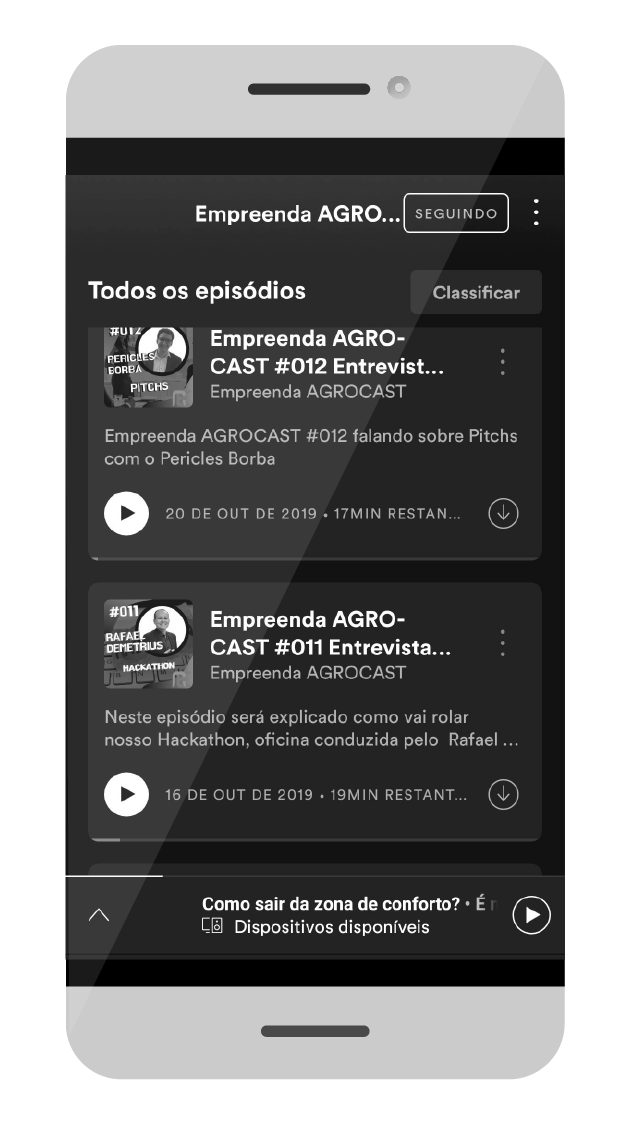
\includegraphics[scale=0.2]{Imagens/aplicativo_4.png}}
\qquad
\subfigure[ref4][Notícias sobre empreendedorismo]{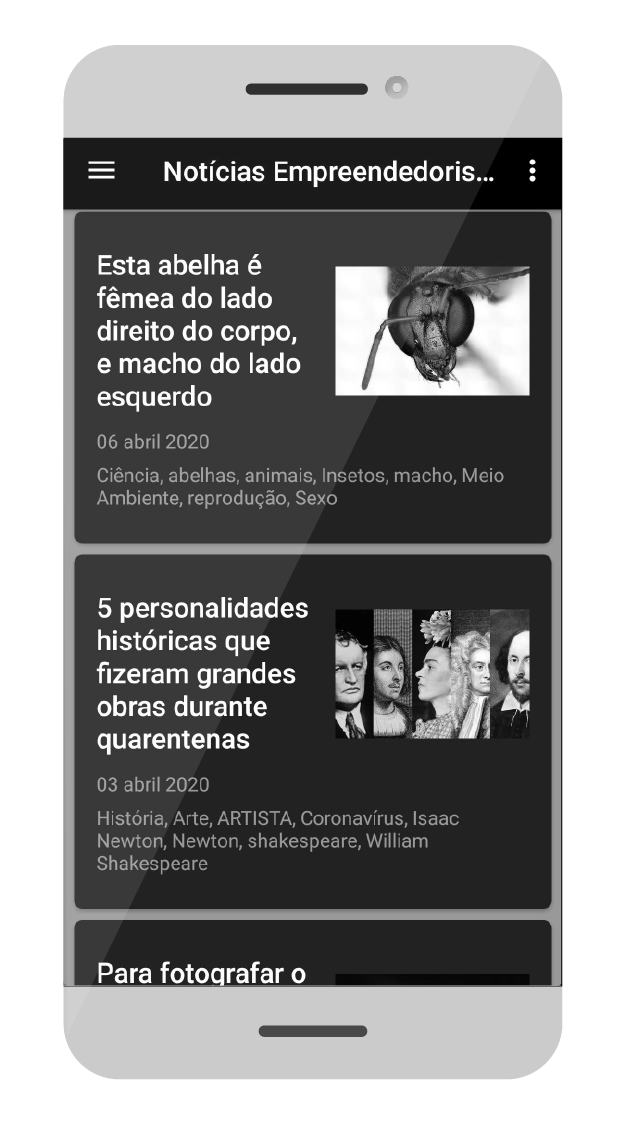
\includegraphics[scale=0.2]{Imagens/aplicativo_5.png}}
\qquad
\subfigure[ref4][Conteúdos escritos]{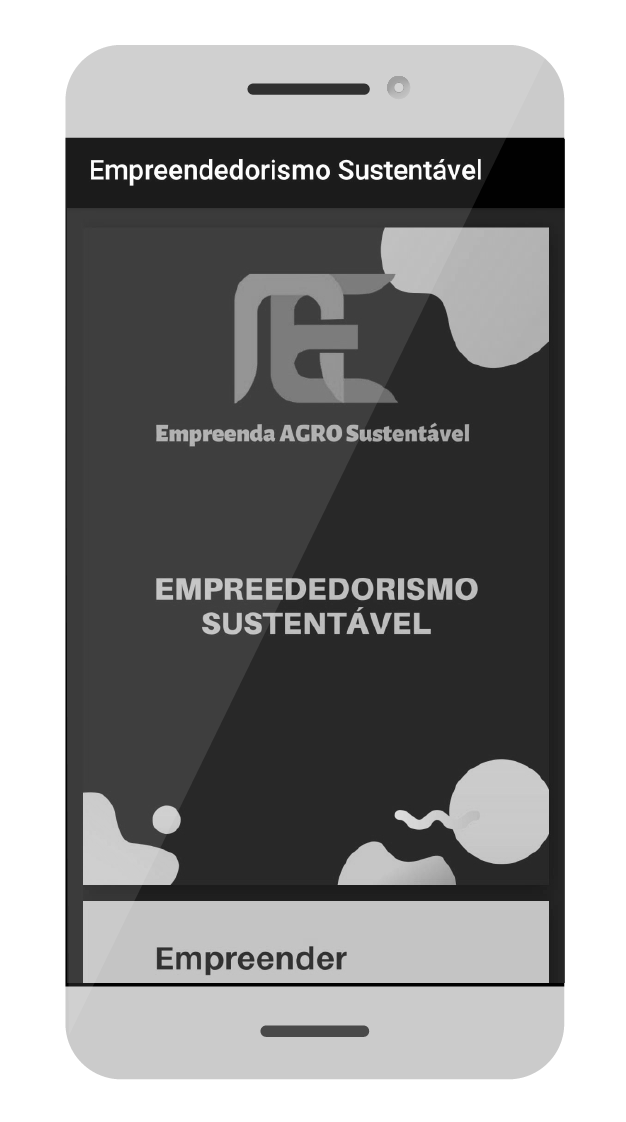
\includegraphics[scale=0.2]{Imagens/aplicativo_6.png}}
\fonte{O Autor}.
\label{figura_44}
\end{figure}


\subsection{Teste de Usabilidade do Aplicativo}

Os principais critérios de inclusão para os usuários testadores foram ter um telefone ‘smartphone’ android e acesso básico a rede de Internet, pois, o aplicativo foi desenvolvido apenas para plataforma Android. A transferência do aplicativo foi disponibilizado de forma grátis por meio da loja de aplicativos Google Play.

Na Figura \ref{figura_43} é possível observar a série temporal dos downloads do aplicativo por meio da plataforma Google Play. A maior quantidade de versões operacionais do sistema Android foi a versão 9.0, tendo alcançando 32 aparelhos ativos desde o início do lançamento (Figura \ref{figura_43}).


\begin{figure}[H]
\caption{\textbf{Série temporal dos dispositivos ativos desde o lançamento no dia 01 de outubro de 2019 até o mês de abril de 2020.}}
\centering
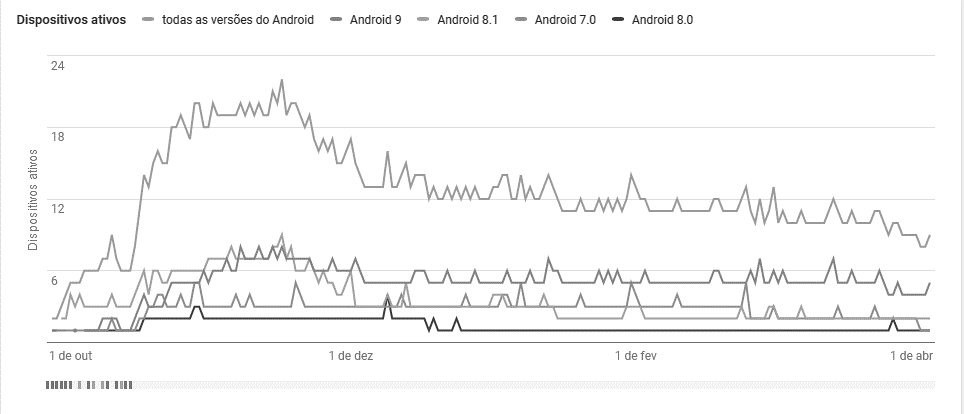
\includegraphics[scale=0.6]{Imagens/dispositivos_instalados.png}
\fonte{ \citeonline{google_developer_google_2020}}
\label{figura_43}
\end{figure}

A entrega do questionário aos usuários através de notificações \textit{Mobile Push} foi realizada ao final do programa. Os usuários participantes do programa foram orientados no começo da disponibilização do aplicativo de como manipular os conteúdos presentes no aplicativo, com a finalidade de observar eventuais falhas durante o uso.
Na fase de testes do aplicativo, entre os 32 participantes, 30 participantes foram capazes de aprender facilmente o uso do aplicativo seguindo as instruções apresentadas nas oficinas de trabalho e apenas 2 tiveram dificuldade no acesso ao conteúdo.

A localização do botão para confirmar a seleção do conteúdo escolhido pelo usuário foi a principal dificuldade relatada por estes dois usuários. A acessibilidade aos recursos, à documentação e às funcionalidades de qualquer aplicativo mobile é um aprendizado natural e leva um certo tempo. Algumas sugestões de melhorias foram indicadas pelos usuários, a saber: remoção deste botão de seleção e fazer com que a função de seleção seja condicionada ao acionamento via Ecrã tátil e a gravação em vídeo de instruções de uso do aplicativo na plataforma de download \textit{Google Play}.

A maioria dos participantes ficou satisfeita quanto ao desempenho do aplicativo como resposta dos recursos e componentes da APP, transição entre telas, uso do menu lateral, e dos botões da tela do aplicativo, assim como dos conteúdos disponibilizados na plataforma, em diferentes formas de acesso (vídeo, áudio e PDF).
Quanto aos erros de desempenho, tais como tempo de atraso na resposta do aplicativo, transição entre telas, uso do teclado deslizante e dos botões da tela do aplicativo, o sistema \textit{Google Vitals} não registrou erros de uso.

O Aplicativo Empreenda Agro Sustentável é uma APP desenvolvida para promoção da educação em empreendedorismo através dos conteúdos dinâmicos direcionados à área de negócios no meio rural, tais como: materiais informativos, videoaulas, ‘podcasts’. O aplicativo também é indicado para profissionais que tenham interesse em aprender mais sobre o desenvolvimento de negócios sustentáveis e escaláveis. Objetiva servir como uma ferramenta para aprimorar os conteúdos ministrados sobre empreendedorismo sustentável no meio rural, fornecendo acesso às informações dos alunos participantes do programa. 

Desta forma os objetivos do aplicativo foram atendidos adequadamente, oferecendo aos usuários participantes a oportunidade de revisar, reforçar e dispor de conteúdos que possam sanar dúvidas após a conclusão do programa. O aplicativo já possui registro no Instituto Nacional de Propriedade Industrial INPI sob número de registro \textbf{BR 51 2019 002657 8} e disponível gratuitamente para testes na loja online Google Play Store.

